\documentclass[]{article}
\usepackage{lmodern}
\usepackage{amssymb,amsmath}
\usepackage{ifxetex,ifluatex}
\usepackage{fixltx2e} % provides \textsubscript
\ifnum 0\ifxetex 1\fi\ifluatex 1\fi=0 % if pdftex
  \usepackage[T1]{fontenc}
  \usepackage[utf8]{inputenc}
\else % if luatex or xelatex
  \ifxetex
    \usepackage{mathspec}
  \else
    \usepackage{fontspec}
  \fi
  \defaultfontfeatures{Ligatures=TeX,Scale=MatchLowercase}
\fi
% use upquote if available, for straight quotes in verbatim environments
\IfFileExists{upquote.sty}{\usepackage{upquote}}{}
% use microtype if available
\IfFileExists{microtype.sty}{%
\usepackage[]{microtype}
\UseMicrotypeSet[protrusion]{basicmath} % disable protrusion for tt fonts
}{}
\PassOptionsToPackage{hyphens}{url} % url is loaded by hyperref
\usepackage[unicode=true]{hyperref}
\hypersetup{
            pdftitle={四元数による回転繰り返し閉路},
            pdfauthor={ryamada},
            pdfborder={0 0 0},
            breaklinks=true}
\urlstyle{same}  % don't use monospace font for urls
\usepackage[margin=1in]{geometry}
\usepackage{color}
\usepackage{fancyvrb}
\newcommand{\VerbBar}{|}
\newcommand{\VERB}{\Verb[commandchars=\\\{\}]}
\DefineVerbatimEnvironment{Highlighting}{Verbatim}{commandchars=\\\{\}}
% Add ',fontsize=\small' for more characters per line
\usepackage{framed}
\definecolor{shadecolor}{RGB}{248,248,248}
\newenvironment{Shaded}{\begin{snugshade}}{\end{snugshade}}
\newcommand{\KeywordTok}[1]{\textcolor[rgb]{0.13,0.29,0.53}{\textbf{#1}}}
\newcommand{\DataTypeTok}[1]{\textcolor[rgb]{0.13,0.29,0.53}{#1}}
\newcommand{\DecValTok}[1]{\textcolor[rgb]{0.00,0.00,0.81}{#1}}
\newcommand{\BaseNTok}[1]{\textcolor[rgb]{0.00,0.00,0.81}{#1}}
\newcommand{\FloatTok}[1]{\textcolor[rgb]{0.00,0.00,0.81}{#1}}
\newcommand{\ConstantTok}[1]{\textcolor[rgb]{0.00,0.00,0.00}{#1}}
\newcommand{\CharTok}[1]{\textcolor[rgb]{0.31,0.60,0.02}{#1}}
\newcommand{\SpecialCharTok}[1]{\textcolor[rgb]{0.00,0.00,0.00}{#1}}
\newcommand{\StringTok}[1]{\textcolor[rgb]{0.31,0.60,0.02}{#1}}
\newcommand{\VerbatimStringTok}[1]{\textcolor[rgb]{0.31,0.60,0.02}{#1}}
\newcommand{\SpecialStringTok}[1]{\textcolor[rgb]{0.31,0.60,0.02}{#1}}
\newcommand{\ImportTok}[1]{#1}
\newcommand{\CommentTok}[1]{\textcolor[rgb]{0.56,0.35,0.01}{\textit{#1}}}
\newcommand{\DocumentationTok}[1]{\textcolor[rgb]{0.56,0.35,0.01}{\textbf{\textit{#1}}}}
\newcommand{\AnnotationTok}[1]{\textcolor[rgb]{0.56,0.35,0.01}{\textbf{\textit{#1}}}}
\newcommand{\CommentVarTok}[1]{\textcolor[rgb]{0.56,0.35,0.01}{\textbf{\textit{#1}}}}
\newcommand{\OtherTok}[1]{\textcolor[rgb]{0.56,0.35,0.01}{#1}}
\newcommand{\FunctionTok}[1]{\textcolor[rgb]{0.00,0.00,0.00}{#1}}
\newcommand{\VariableTok}[1]{\textcolor[rgb]{0.00,0.00,0.00}{#1}}
\newcommand{\ControlFlowTok}[1]{\textcolor[rgb]{0.13,0.29,0.53}{\textbf{#1}}}
\newcommand{\OperatorTok}[1]{\textcolor[rgb]{0.81,0.36,0.00}{\textbf{#1}}}
\newcommand{\BuiltInTok}[1]{#1}
\newcommand{\ExtensionTok}[1]{#1}
\newcommand{\PreprocessorTok}[1]{\textcolor[rgb]{0.56,0.35,0.01}{\textit{#1}}}
\newcommand{\AttributeTok}[1]{\textcolor[rgb]{0.77,0.63,0.00}{#1}}
\newcommand{\RegionMarkerTok}[1]{#1}
\newcommand{\InformationTok}[1]{\textcolor[rgb]{0.56,0.35,0.01}{\textbf{\textit{#1}}}}
\newcommand{\WarningTok}[1]{\textcolor[rgb]{0.56,0.35,0.01}{\textbf{\textit{#1}}}}
\newcommand{\AlertTok}[1]{\textcolor[rgb]{0.94,0.16,0.16}{#1}}
\newcommand{\ErrorTok}[1]{\textcolor[rgb]{0.64,0.00,0.00}{\textbf{#1}}}
\newcommand{\NormalTok}[1]{#1}
\usepackage{graphicx,grffile}
\makeatletter
\def\maxwidth{\ifdim\Gin@nat@width>\linewidth\linewidth\else\Gin@nat@width\fi}
\def\maxheight{\ifdim\Gin@nat@height>\textheight\textheight\else\Gin@nat@height\fi}
\makeatother
% Scale images if necessary, so that they will not overflow the page
% margins by default, and it is still possible to overwrite the defaults
% using explicit options in \includegraphics[width, height, ...]{}
\setkeys{Gin}{width=\maxwidth,height=\maxheight,keepaspectratio}
\IfFileExists{parskip.sty}{%
\usepackage{parskip}
}{% else
\setlength{\parindent}{0pt}
\setlength{\parskip}{6pt plus 2pt minus 1pt}
}
\setlength{\emergencystretch}{3em}  % prevent overfull lines
\providecommand{\tightlist}{%
  \setlength{\itemsep}{0pt}\setlength{\parskip}{0pt}}
\setcounter{secnumdepth}{0}
% Redefines (sub)paragraphs to behave more like sections
\ifx\paragraph\undefined\else
\let\oldparagraph\paragraph
\renewcommand{\paragraph}[1]{\oldparagraph{#1}\mbox{}}
\fi
\ifx\subparagraph\undefined\else
\let\oldsubparagraph\subparagraph
\renewcommand{\subparagraph}[1]{\oldsubparagraph{#1}\mbox{}}
\fi

% set default figure placement to htbp
\makeatletter
\def\fps@figure{htbp}
\makeatother


\title{四元数による回転繰り返し閉路}
\author{ryamada}
\date{2020/6/7}

\begin{document}
\maketitle

\subsection{3次元空間の回転と四元数}\label{ux6b21ux5143ux7a7aux9593ux306eux56deux8ee2ux3068ux56dbux5143ux6570}

単位四元数\(q = \cos{\theta/2} \times \mathbf{1} + \sin{\theta/2} \times (x \mathbf{i} + y \mathbf{j} + z \mathbf{k});x^2+y^2+z^2=1\)
を用いると、
3次元空間のベクトル\(v=(v_x,v_y,v_z)\)を軸\((x,y,z)\)の周りに角\(\theta\)で回転してできるベクトル\(v'=(v_x',v_y',v_z')\)は

\[
v_x' \mathbf{i} + v_y' \mathbf{j} + v_z' \mathbf{k} = q \times (v_x \mathbf{i} + v_y \mathbf{j} + v_z \mathbf{k}) \bar{q}
\]
ただし、\(\bar{q}=conj(q) = \cos{\theta/2} \times \mathbf{1} - \sin{\theta/2} \times (x \mathbf{i} + y \mathbf{j} + z \mathbf{k})\)

で得られる。

\begin{Shaded}
\begin{Highlighting}[]
\KeywordTok{library}\NormalTok{(onion)}
\end{Highlighting}
\end{Shaded}

\begin{Shaded}
\begin{Highlighting}[]
\NormalTok{theta <-}\StringTok{ }\NormalTok{pi}\OperatorTok{/}\DecValTok{3}
\NormalTok{xyz <-}\StringTok{ }\KeywordTok{c}\NormalTok{(}\DecValTok{1}\NormalTok{,}\DecValTok{0}\NormalTok{,}\DecValTok{0}\NormalTok{)}
\NormalTok{v <-}\StringTok{ }\KeywordTok{c}\NormalTok{(}\DecValTok{0}\NormalTok{,}\DecValTok{1}\NormalTok{,}\DecValTok{0}\NormalTok{)}

\NormalTok{q <-}\StringTok{ }\KeywordTok{cos}\NormalTok{(theta}\OperatorTok{/}\DecValTok{2}\NormalTok{) }\OperatorTok{+}\StringTok{ }\KeywordTok{sin}\NormalTok{(theta}\OperatorTok{/}\DecValTok{2}\NormalTok{)}\OperatorTok{*}\NormalTok{(xyz[}\DecValTok{1}\NormalTok{]}\OperatorTok{*}\NormalTok{Hi }\OperatorTok{+}\StringTok{ }\NormalTok{xyz[}\DecValTok{2}\NormalTok{]}\OperatorTok{*}\NormalTok{Hj }\OperatorTok{+}\StringTok{ }\NormalTok{xyz[}\DecValTok{3}\NormalTok{]}\OperatorTok{*}\NormalTok{Hk)}
\NormalTok{v.q <-}\StringTok{ }\NormalTok{v[}\DecValTok{1}\NormalTok{]}\OperatorTok{*}\NormalTok{Hi }\OperatorTok{+}\StringTok{ }\NormalTok{v[}\DecValTok{2}\NormalTok{]}\OperatorTok{*}\NormalTok{Hj }\OperatorTok{+}\StringTok{ }\NormalTok{v[}\DecValTok{3}\NormalTok{]}\OperatorTok{*}\NormalTok{Hk}
\NormalTok{v. <-}\StringTok{ }\NormalTok{q }\OperatorTok{*}\StringTok{ }\NormalTok{v.q }\OperatorTok{*}\StringTok{ }\KeywordTok{Conj}\NormalTok{(q)}
\NormalTok{v.}
\end{Highlighting}
\end{Shaded}

\begin{verbatim}
##          [1]
## Re 0.0000000
## i  0.0000000
## j  0.5000000
## k  0.8660254
\end{verbatim}

\begin{Shaded}
\begin{Highlighting}[]
\KeywordTok{Mod}\NormalTok{(v.)}
\end{Highlighting}
\end{Shaded}

\begin{verbatim}
## [1] 1
\end{verbatim}

\begin{Shaded}
\begin{Highlighting}[]
\KeywordTok{acos}\NormalTok{(}\KeywordTok{sum}\NormalTok{(v}\OperatorTok{*}\KeywordTok{c}\NormalTok{(}\KeywordTok{i}\NormalTok{(v.),}\KeywordTok{j}\NormalTok{(v.),}\KeywordTok{k}\NormalTok{(v.))))}\OperatorTok{/}\NormalTok{pi }\CommentTok{# 内積を計算して、角度を求める、1/3 pi である}
\end{Highlighting}
\end{Shaded}

\begin{verbatim}
## [1] 0.3333333
\end{verbatim}

\subsection{回転四元数に対応する回転行列}\label{ux56deux8ee2ux56dbux5143ux6570ux306bux5bfeux5fdcux3059ux308bux56deux8ee2ux884cux5217}

\begin{Shaded}
\begin{Highlighting}[]
\KeywordTok{library}\NormalTok{(onion)}
\NormalTok{tmp <-}\StringTok{ }\KeywordTok{rnorm}\NormalTok{(}\DecValTok{4}\NormalTok{)}
\NormalTok{tmp <-}\StringTok{ }\NormalTok{tmp}\OperatorTok{/}\KeywordTok{sqrt}\NormalTok{(}\KeywordTok{sum}\NormalTok{(tmp}\OperatorTok{^}\DecValTok{2}\NormalTok{))}
\NormalTok{q <-}\StringTok{ }\NormalTok{tmp[}\DecValTok{1}\NormalTok{] }\OperatorTok{+}\StringTok{ }\NormalTok{tmp[}\DecValTok{2}\NormalTok{]}\OperatorTok{*}\NormalTok{Hi }\OperatorTok{+}\StringTok{ }\NormalTok{tmp[}\DecValTok{3}\NormalTok{] }\OperatorTok{*}\StringTok{ }\NormalTok{Hj }\OperatorTok{+}\StringTok{ }\NormalTok{tmp[}\DecValTok{4}\NormalTok{] }\OperatorTok{*}\StringTok{ }\NormalTok{Hk}

\NormalTok{v <-}\StringTok{ }\KeywordTok{rnorm}\NormalTok{(}\DecValTok{3}\NormalTok{)}
\NormalTok{v.q <-}\StringTok{ }\NormalTok{v[}\DecValTok{1}\NormalTok{]}\OperatorTok{*}\NormalTok{Hi }\OperatorTok{+}\StringTok{ }\NormalTok{v[}\DecValTok{2}\NormalTok{] }\OperatorTok{*}\StringTok{ }\NormalTok{Hj }\OperatorTok{+}\StringTok{ }\NormalTok{v[}\DecValTok{3}\NormalTok{] }\OperatorTok{*}\StringTok{ }\NormalTok{Hk}

\NormalTok{v. <-}\StringTok{ }\NormalTok{q }\OperatorTok{*}\StringTok{ }\NormalTok{v.q }\OperatorTok{*}\StringTok{ }\KeywordTok{Conj}\NormalTok{(q)}



\NormalTok{A <-}\StringTok{ }\KeywordTok{Re}\NormalTok{(q)}
\NormalTok{B <-}\StringTok{ }\KeywordTok{i}\NormalTok{(q)}
\NormalTok{C <-}\StringTok{ }\KeywordTok{j}\NormalTok{(q)}
\NormalTok{D <-}\StringTok{ }\KeywordTok{k}\NormalTok{(q)}
\NormalTok{R <-}\StringTok{ }\KeywordTok{matrix}\NormalTok{(}\KeywordTok{c}\NormalTok{(A}\OperatorTok{^}\DecValTok{2}\OperatorTok{+}\NormalTok{B}\OperatorTok{^}\DecValTok{2}\OperatorTok{-}\NormalTok{C}\OperatorTok{^}\DecValTok{2}\OperatorTok{-}\NormalTok{D}\OperatorTok{^}\DecValTok{2}\NormalTok{,}\DecValTok{2}\OperatorTok{*}\NormalTok{(}\OperatorTok{-}\NormalTok{A}\OperatorTok{*}\NormalTok{D}\OperatorTok{+}\NormalTok{B}\OperatorTok{*}\NormalTok{C),}\DecValTok{2}\OperatorTok{*}\NormalTok{(A}\OperatorTok{*}\NormalTok{C}\OperatorTok{+}\NormalTok{B}\OperatorTok{*}\NormalTok{D),}\DecValTok{2}\OperatorTok{*}\NormalTok{(A}\OperatorTok{*}\NormalTok{D}\OperatorTok{+}\NormalTok{B}\OperatorTok{*}\NormalTok{C),A}\OperatorTok{^}\DecValTok{2}\OperatorTok{-}\NormalTok{B}\OperatorTok{^}\DecValTok{2}\OperatorTok{+}\NormalTok{C}\OperatorTok{^}\DecValTok{2}\OperatorTok{-}\NormalTok{D}\OperatorTok{^}\DecValTok{2}\NormalTok{,}\DecValTok{2}\OperatorTok{*}\NormalTok{(}\OperatorTok{-}\NormalTok{A}\OperatorTok{*}\NormalTok{B}\OperatorTok{+}\NormalTok{C}\OperatorTok{*}\NormalTok{D),}\DecValTok{2}\OperatorTok{*}\NormalTok{(}\OperatorTok{-}\NormalTok{A}\OperatorTok{*}\NormalTok{C}\OperatorTok{+}\NormalTok{B}\OperatorTok{*}\NormalTok{D),}\DecValTok{2}\OperatorTok{*}\NormalTok{(A}\OperatorTok{*}\NormalTok{B}\OperatorTok{+}\NormalTok{C}\OperatorTok{*}\NormalTok{D),A}\OperatorTok{^}\DecValTok{2}\OperatorTok{-}\NormalTok{B}\OperatorTok{^}\DecValTok{2}\OperatorTok{-}\NormalTok{C}\OperatorTok{^}\DecValTok{2}\OperatorTok{+}\NormalTok{D}\OperatorTok{^}\DecValTok{2}\NormalTok{),}\DataTypeTok{byrow=}\OtherTok{TRUE}\NormalTok{,}\DecValTok{3}\NormalTok{,}\DecValTok{3}\NormalTok{)}

\NormalTok{R}
\end{Highlighting}
\end{Shaded}

\begin{verbatim}
##             [,1]      [,2]        [,3]
## [1,] -0.83551353 0.5430870  0.08350827
## [2,]  0.54662358 0.8060810  0.22679522
## [3,]  0.05585511 0.2351381 -0.97035576
\end{verbatim}

\begin{Shaded}
\begin{Highlighting}[]
\NormalTok{R }\OperatorTok\StringTok{ }\KeywordTok{matrix}\NormalTok{(v,}\DataTypeTok{ncol=}\DecValTok{1}\NormalTok{)}
\end{Highlighting}
\end{Shaded}

\begin{verbatim}
##            [,1]
## [1,] -2.0353202
## [2,] -0.9563953
## [3,] -0.5557610
\end{verbatim}

\begin{Shaded}
\begin{Highlighting}[]
\NormalTok{v.}
\end{Highlighting}
\end{Shaded}

\begin{verbatim}
##              [1]
## Re  5.551115e-17
## i  -2.035320e+00
## j  -9.563953e-01
## k  -5.557610e-01
\end{verbatim}

\begin{Shaded}
\begin{Highlighting}[]
\NormalTok{my.rot.mat <-}\StringTok{ }\ControlFlowTok{function}\NormalTok{(V,theta)\{}
\NormalTok{  V <-}\StringTok{ }\NormalTok{V}\OperatorTok{/}\KeywordTok{sqrt}\NormalTok{(}\KeywordTok{sum}\NormalTok{(V}\OperatorTok{^}\DecValTok{2}\NormalTok{))}
\NormalTok{  A <-}\StringTok{ }\KeywordTok{cos}\NormalTok{(theta}\OperatorTok{/}\DecValTok{2}\NormalTok{) }
\NormalTok{  B <-}\StringTok{ }\KeywordTok{sin}\NormalTok{(theta}\OperatorTok{/}\DecValTok{2}\NormalTok{) }\OperatorTok{*}\StringTok{ }\NormalTok{V[}\DecValTok{1}\NormalTok{]}
\NormalTok{  C <-}\StringTok{ }\KeywordTok{sin}\NormalTok{(theta}\OperatorTok{/}\DecValTok{2}\NormalTok{) }\OperatorTok{*}\StringTok{ }\NormalTok{V[}\DecValTok{2}\NormalTok{]}
\NormalTok{  D <-}\StringTok{ }\KeywordTok{sin}\NormalTok{(theta}\OperatorTok{/}\DecValTok{2}\NormalTok{) }\OperatorTok{*}\StringTok{ }\NormalTok{V[}\DecValTok{3}\NormalTok{]}
\NormalTok{  R <-}\StringTok{ }\KeywordTok{matrix}\NormalTok{(}\KeywordTok{c}\NormalTok{(A}\OperatorTok{^}\DecValTok{2}\OperatorTok{+}\NormalTok{B}\OperatorTok{^}\DecValTok{2}\OperatorTok{-}\NormalTok{C}\OperatorTok{^}\DecValTok{2}\OperatorTok{-}\NormalTok{D}\OperatorTok{^}\DecValTok{2}\NormalTok{,}\DecValTok{2}\OperatorTok{*}\NormalTok{(}\OperatorTok{-}\NormalTok{A}\OperatorTok{*}\NormalTok{D}\OperatorTok{+}\NormalTok{B}\OperatorTok{*}\NormalTok{C),}\DecValTok{2}\OperatorTok{*}\NormalTok{(A}\OperatorTok{*}\NormalTok{C}\OperatorTok{+}\NormalTok{B}\OperatorTok{*}\NormalTok{D),}\DecValTok{2}\OperatorTok{*}\NormalTok{(A}\OperatorTok{*}\NormalTok{D}\OperatorTok{+}\NormalTok{B}\OperatorTok{*}\NormalTok{C),A}\OperatorTok{^}\DecValTok{2}\OperatorTok{-}\NormalTok{B}\OperatorTok{^}\DecValTok{2}\OperatorTok{+}\NormalTok{C}\OperatorTok{^}\DecValTok{2}\OperatorTok{-}\NormalTok{D}\OperatorTok{^}\DecValTok{2}\NormalTok{,}\DecValTok{2}\OperatorTok{*}\NormalTok{(}\OperatorTok{-}\NormalTok{A}\OperatorTok{*}\NormalTok{B}\OperatorTok{+}\NormalTok{C}\OperatorTok{*}\NormalTok{D),}\DecValTok{2}\OperatorTok{*}\NormalTok{(}\OperatorTok{-}\NormalTok{A}\OperatorTok{*}\NormalTok{C}\OperatorTok{+}\NormalTok{B}\OperatorTok{*}\NormalTok{D),}\DecValTok{2}\OperatorTok{*}\NormalTok{(A}\OperatorTok{*}\NormalTok{B}\OperatorTok{+}\NormalTok{C}\OperatorTok{*}\NormalTok{D),A}\OperatorTok{^}\DecValTok{2}\OperatorTok{-}\NormalTok{B}\OperatorTok{^}\DecValTok{2}\OperatorTok{-}\NormalTok{C}\OperatorTok{^}\DecValTok{2}\OperatorTok{+}\NormalTok{D}\OperatorTok{^}\DecValTok{2}\NormalTok{),}\DataTypeTok{byrow=}\OtherTok{TRUE}\NormalTok{,}\DecValTok{3}\NormalTok{,}\DecValTok{3}\NormalTok{)}
  \KeywordTok{return}\NormalTok{(R) }
\NormalTok{\}}
\NormalTok{my.function.tri.rot <-}\StringTok{ }\ControlFlowTok{function}\NormalTok{(A,N,theta,}\DataTypeTok{zigzag=}\OtherTok{FALSE}\NormalTok{)\{ }
\NormalTok{  psi <-}\StringTok{ }\NormalTok{pi}\OperatorTok{/}\DecValTok{3}
  \ControlFlowTok{if}\NormalTok{(zigzag)\{}
\NormalTok{    psi <-}\StringTok{ }\OperatorTok{-}\StringTok{ }\NormalTok{pi }\OperatorTok{/}\StringTok{ }\DecValTok{3}
\NormalTok{  \}}
\NormalTok{  R <-}\StringTok{ }\KeywordTok{my.rot.mat}\NormalTok{(A,theta)}
\NormalTok{  N.new <-}\StringTok{ }\NormalTok{R }\OperatorTok\StringTok{ }\KeywordTok{matrix}\NormalTok{(N,}\DataTypeTok{ncol=}\DecValTok{1}\NormalTok{)}
  \CommentTok{#R2 <- my.rot.mat(N.new,pi/3)}
\NormalTok{  R2 <-}\StringTok{ }\KeywordTok{my.rot.mat}\NormalTok{(N.new,psi)}
\NormalTok{  A.new <-}\StringTok{ }\NormalTok{R2 }\OperatorTok\StringTok{ }\KeywordTok{matrix}\NormalTok{(A,}\DataTypeTok{ncol=}\DecValTok{1}\NormalTok{) }
  \KeywordTok{return}\NormalTok{(}\KeywordTok{list}\NormalTok{(}\DataTypeTok{N=}\NormalTok{N.new,}\DataTypeTok{A=}\NormalTok{A.new)) }
\NormalTok{\}}

\NormalTok{my.function.tri.rot.series <-}\StringTok{ }\ControlFlowTok{function}\NormalTok{(}\DataTypeTok{A=}\KeywordTok{c}\NormalTok{(}\DecValTok{1}\NormalTok{,}\DecValTok{0}\NormalTok{,}\DecValTok{0}\NormalTok{),}\DataTypeTok{N=}\KeywordTok{c}\NormalTok{(}\DecValTok{0}\NormalTok{,}\DecValTok{0}\NormalTok{,}\DecValTok{1}\NormalTok{),thetas,}\DataTypeTok{zigzag=}\OtherTok{FALSE}\NormalTok{)\{}
\NormalTok{  As <-}\StringTok{ }\NormalTok{Ns <-}\StringTok{ }\KeywordTok{matrix}\NormalTok{(}\DecValTok{0}\NormalTok{,}\KeywordTok{length}\NormalTok{(thetas)}\OperatorTok{+}\DecValTok{1}\NormalTok{,}\KeywordTok{length}\NormalTok{(A))}
\NormalTok{  As[}\DecValTok{1}\NormalTok{,] <-}\StringTok{ }\NormalTok{A}
\NormalTok{  Ns[}\DecValTok{1}\NormalTok{,] <-}\StringTok{ }\NormalTok{N}
  \ControlFlowTok{for}\NormalTok{(i }\ControlFlowTok{in} \DecValTok{1}\OperatorTok{:}\KeywordTok{length}\NormalTok{(thetas))\{}
    \ControlFlowTok{if}\NormalTok{(i }\OperatorTok\StringTok{ }\DecValTok{2} \OperatorTok{==}\StringTok{ }\DecValTok{0}\NormalTok{)\{}
\NormalTok{      tmp <-}\StringTok{ }\KeywordTok{my.function.tri.rot}\NormalTok{(As[i,],Ns[i,],thetas[i],}\DataTypeTok{zigzag=}\OtherTok{FALSE}\NormalTok{)}
\NormalTok{    \}}\ControlFlowTok{else}\NormalTok{\{}
\NormalTok{      tmp <-}\StringTok{ }\KeywordTok{my.function.tri.rot}\NormalTok{(As[i,],Ns[i,],thetas[i],}\DataTypeTok{zigzag=}\NormalTok{zigzag)}
\NormalTok{    \}}
    

    
\NormalTok{    As[i}\OperatorTok{+}\DecValTok{1}\NormalTok{,] <-}\StringTok{ }\NormalTok{tmp}\OperatorTok{$}\NormalTok{A}
\NormalTok{    Ns[i}\OperatorTok{+}\DecValTok{1}\NormalTok{,] <-}\StringTok{ }\NormalTok{tmp}\OperatorTok{$}\NormalTok{N}
\NormalTok{  \}}
  \KeywordTok{return}\NormalTok{(}\KeywordTok{list}\NormalTok{(}\DataTypeTok{As=}\NormalTok{As,}\DataTypeTok{Ns=}\NormalTok{Ns,}\DataTypeTok{k=}\KeywordTok{length}\NormalTok{(thetas)))}
\NormalTok{\}}
\end{Highlighting}
\end{Shaded}

\subsection{6個の正三角形を平面に並べて正六角形を作る}\label{ux500bux306eux6b63ux4e09ux89d2ux5f62ux3092ux5e73ux9762ux306bux4e26ux3079ux3066ux6b63ux516dux89d2ux5f62ux3092ux4f5cux308b}

\begin{Shaded}
\begin{Highlighting}[]
\NormalTok{A1 <-}\StringTok{ }\KeywordTok{c}\NormalTok{(}\DecValTok{1}\NormalTok{,}\DecValTok{0}\NormalTok{,}\DecValTok{0}\NormalTok{)}
\NormalTok{N1 <-}\StringTok{ }\KeywordTok{c}\NormalTok{(}\DecValTok{0}\NormalTok{,}\DecValTok{0}\NormalTok{,}\DecValTok{1}\NormalTok{)}

\NormalTok{k <-}\StringTok{ }\DecValTok{6}
\NormalTok{thetas <-}\StringTok{ }\KeywordTok{rep}\NormalTok{(}\DecValTok{0}\NormalTok{,k) }\CommentTok{# 回転角は0ばかり}

\NormalTok{ANs <-}\StringTok{ }\KeywordTok{list}\NormalTok{()}
\NormalTok{ANs[[}\DecValTok{1}\NormalTok{]] <-}\StringTok{ }\KeywordTok{list}\NormalTok{(}\DataTypeTok{A=}\NormalTok{A1,}\DataTypeTok{N=}\NormalTok{N1)}
\ControlFlowTok{for}\NormalTok{(i }\ControlFlowTok{in} \DecValTok{1}\OperatorTok{:}\NormalTok{k)\{}
\NormalTok{  tmp <-}\StringTok{ }\KeywordTok{my.function.tri.rot}\NormalTok{(ANs[[i]]}\OperatorTok{$}\NormalTok{A,ANs[[i]]}\OperatorTok{$}\NormalTok{N,thetas[i])}
\NormalTok{  ANs[[i}\OperatorTok{+}\DecValTok{1}\NormalTok{]] <-}\StringTok{ }\KeywordTok{list}\NormalTok{(}\DataTypeTok{A=}\NormalTok{tmp}\OperatorTok{$}\NormalTok{A,}\DataTypeTok{N=}\NormalTok{tmp}\OperatorTok{$}\NormalTok{N)}
\NormalTok{\}}
\CommentTok{# 確かに、辺ベクトル、法線ベクトルとが元に戻っている}
\NormalTok{ANs[[}\DecValTok{1}\NormalTok{]][[}\DecValTok{1}\NormalTok{]] }\OperatorTok{-}\StringTok{ }\NormalTok{ANs[[k}\OperatorTok{+}\DecValTok{1}\NormalTok{]][[}\DecValTok{1}\NormalTok{]]}
\end{Highlighting}
\end{Shaded}

\begin{verbatim}
##               [,1]
## [1,] -4.440892e-16
## [2,]  1.276756e-15
## [3,]  0.000000e+00
\end{verbatim}

\begin{Shaded}
\begin{Highlighting}[]
\NormalTok{ANs[[}\DecValTok{1}\NormalTok{]][[}\DecValTok{2}\NormalTok{]] }\OperatorTok{-}\StringTok{ }\NormalTok{ANs[[k}\OperatorTok{+}\DecValTok{1}\NormalTok{]][[}\DecValTok{2}\NormalTok{]] }
\end{Highlighting}
\end{Shaded}

\begin{verbatim}
##      [,1]
## [1,]    0
## [2,]    0
## [3,]    0
\end{verbatim}

\subsection{対称性のある並べ方}\label{ux5bfeux79f0ux6027ux306eux3042ux308bux4e26ux3079ux65b9}

\subsubsection{2個、3個、\ldots{}、6個までは、ある同一角で連結して閉じさせることができる}\label{ux500b3ux500b6ux500bux307eux3067ux306fux3042ux308bux540cux4e00ux89d2ux3067ux9023ux7d50ux3057ux3066ux9589ux3058ux3055ux305bux308bux3053ux3068ux304cux3067ux304dux308b}

その角が幾つなのか、計算機的に算出してみる。

角度を細かく変化させ、一周してきて、辺ベクトルと法線ベクトルとが一致する角度(の0より大きい)最小値を探索する。

まずは、2個。

これは、2つの正三角形の表裏貼り合わせ。 「正解」は\(\pi\)。

最初の辺と周回してきた辺との内積が1で、最初の法線ベクトルと周回してきた法線ベクトルとの内積が1であるような、角度が、閉じさせる角度。

3個は正四面体、4個はピラミッド、5個は正二十面体の1頂点を巡る5面、そして6個は平面。

7個以上になると、ある等角度で接続していくと「余って」しまうので、以下の例では、2周して閉じる場合が算出されている。

グラフ表示は、面の数ごとに2つ描いている。

左側のパネルは、横軸に回転角(単位\(\pi\))で、1周して戻ってきた、辺ベクトルと最初の辺ベクトルとの内積、最初と1周後の法線ベクトルの内積とを縦軸に取っている。

両方が揃って、内積1になる角度が、うまく閉じた場合に相当する。

うまく閉じる角度のうち、最小のものが、求める角度。

右側のパネルは、辺ベクトル内積と法線ベクトル内積との2次元変化の様子を表す。点(1,1)に到達すれば、それは、うまく閉じることを意味する。

正三角形の個数が増えると、うまく閉じる角度が複数通り現れる様子が、点(1,1)に繰り返し曲線が戻ることから読み取れる。

\begin{Shaded}
\begin{Highlighting}[]
\NormalTok{my.tri.cycle <-}\StringTok{ }\ControlFlowTok{function}\NormalTok{(k, }\DataTypeTok{s=}\DecValTok{3}\NormalTok{,}\DataTypeTok{numtheta =} \DecValTok{1003}\NormalTok{,}\DataTypeTok{max.theta =} \DecValTok{2} \OperatorTok{*}\StringTok{ }\NormalTok{pi }\OperatorTok{*}\StringTok{ }\DecValTok{1}\NormalTok{,}\DataTypeTok{sign.alt=}\OtherTok{FALSE}\NormalTok{)\{}
\NormalTok{  theta.list <-}\StringTok{ }\KeywordTok{seq}\NormalTok{(}\DataTypeTok{from=}\DecValTok{0}\NormalTok{,}\DataTypeTok{to=}\NormalTok{max.theta,}\DataTypeTok{length=}\NormalTok{numtheta)}
  
\NormalTok{  cosAs <-}\StringTok{ }\NormalTok{cosNs <-}\StringTok{ }\KeywordTok{rep}\NormalTok{(}\DecValTok{0}\NormalTok{,}\KeywordTok{length}\NormalTok{(theta.list))}
\NormalTok{  cosANs.sq <-}\StringTok{ }\NormalTok{cosAs}
  \ControlFlowTok{for}\NormalTok{(ii }\ControlFlowTok{in} \DecValTok{1}\OperatorTok{:}\KeywordTok{length}\NormalTok{(theta.list))\{}
\NormalTok{    thetas <-}\StringTok{ }\KeywordTok{rep}\NormalTok{(theta.list[ii],k)}
    \ControlFlowTok{if}\NormalTok{(sign.alt)\{}
\NormalTok{      thetas <-}\StringTok{ }\NormalTok{thetas }\OperatorTok{*}\StringTok{ }\NormalTok{(}\OperatorTok{-}\DecValTok{1}\NormalTok{)}\OperatorTok{^}\NormalTok{(}\DecValTok{1}\OperatorTok{:}\KeywordTok{length}\NormalTok{(thetas)) }\OperatorTok{*}\StringTok{ }\NormalTok{(}\OperatorTok{-}\DecValTok{1}\NormalTok{)}
\NormalTok{    \}}
\NormalTok{    ANs <-}\StringTok{ }\KeywordTok{list}\NormalTok{()}
\NormalTok{    ANs[[}\DecValTok{1}\NormalTok{]] <-}\StringTok{ }\KeywordTok{list}\NormalTok{(}\DataTypeTok{A=}\NormalTok{A1,}\DataTypeTok{N=}\NormalTok{N1)}
    \ControlFlowTok{for}\NormalTok{(i }\ControlFlowTok{in} \DecValTok{1}\OperatorTok{:}\NormalTok{k)\{}
\NormalTok{      tmp <-}\StringTok{ }\KeywordTok{my.function.tri.rot}\NormalTok{(ANs[[i]]}\OperatorTok{$}\NormalTok{A,ANs[[i]]}\OperatorTok{$}\NormalTok{N,thetas[i])}
\NormalTok{      ANs[[i}\OperatorTok{+}\DecValTok{1}\NormalTok{]] <-}\StringTok{ }\KeywordTok{list}\NormalTok{(}\DataTypeTok{A=}\NormalTok{tmp}\OperatorTok{$}\NormalTok{A,}\DataTypeTok{N=}\NormalTok{tmp}\OperatorTok{$}\NormalTok{N)}
\NormalTok{    \}}
\NormalTok{    cosAs[ii] <-}\StringTok{ }\KeywordTok{sum}\NormalTok{(ANs[[}\DecValTok{1}\NormalTok{]][[}\DecValTok{1}\NormalTok{]] }\OperatorTok{*}\StringTok{ }\NormalTok{ANs[[k}\OperatorTok{+}\DecValTok{1}\NormalTok{]][[}\DecValTok{1}\NormalTok{]])}
\NormalTok{    cosNs[ii] <-}\StringTok{ }\KeywordTok{sum}\NormalTok{(ANs[[}\DecValTok{1}\NormalTok{]][[}\DecValTok{2}\NormalTok{]] }\OperatorTok{*}\StringTok{ }\NormalTok{ANs[[k}\OperatorTok{+}\DecValTok{1}\NormalTok{]][[}\DecValTok{2}\NormalTok{]]) }
  
\NormalTok{  \}}
  
  \CommentTok{#theta.list[which((abs(cosAs-1) + abs(cosNs-1) < 10^(-4)) & ((abs(cosAs-1) + abs(cosNs-1) == min(abs(cosAs-1) + abs(cosNs-1)))))]}
\NormalTok{  cosANs <-}\StringTok{ }\KeywordTok{cbind}\NormalTok{(cosAs,cosNs)}
\NormalTok{  cosANs.sum <-}\StringTok{ }\KeywordTok{apply}\NormalTok{(cosANs,}\DecValTok{1}\NormalTok{,sum)}
\NormalTok{  best.theta <-}\StringTok{ }\NormalTok{theta.list[}\KeywordTok{which}\NormalTok{(cosANs.sum }\OperatorTok{>}\StringTok{ }\DecValTok{2}\OperatorTok{-}\DecValTok{10}\OperatorTok{^}\NormalTok{(}\OperatorTok{-}\NormalTok{s))][}\DecValTok{1}\NormalTok{]}
  
  
  \KeywordTok{par}\NormalTok{(}\DataTypeTok{mfcol=}\KeywordTok{c}\NormalTok{(}\DecValTok{1}\NormalTok{,}\DecValTok{2}\NormalTok{)) }
  \KeywordTok{matplot}\NormalTok{(theta.list}\OperatorTok{/}\NormalTok{pi,}\KeywordTok{cbind}\NormalTok{(cosAs,cosNs),}\DataTypeTok{type=}\StringTok{"l"}\NormalTok{,}\DataTypeTok{xlab=}\StringTok{"angle(unit=pi)"}\NormalTok{,}\DataTypeTok{ylab=}\StringTok{"cosines of edge vectors and normal vectors"}\NormalTok{,}\DataTypeTok{main =} \KeywordTok{paste}\NormalTok{(}\StringTok{"k="}\NormalTok{,k))}
  \KeywordTok{abline}\NormalTok{(}\DataTypeTok{h=}\DecValTok{1}\NormalTok{,}\DataTypeTok{col=}\DecValTok{3}\NormalTok{)}
  \KeywordTok{abline}\NormalTok{(}\DataTypeTok{v=}\NormalTok{best.theta}\OperatorTok{/}\NormalTok{pi,}\DataTypeTok{col=}\DecValTok{3}\NormalTok{)}
  \KeywordTok{plot}\NormalTok{(cosAs,cosNs,}\DataTypeTok{type=}\StringTok{"l"}\NormalTok{,}\DataTypeTok{xlab=}\StringTok{"cos(edge_vecs)"}\NormalTok{,}\DataTypeTok{ylab=}\StringTok{"cos(norm_vecs)"}\NormalTok{)}
  \KeywordTok{points}\NormalTok{(}\KeywordTok{c}\NormalTok{(}\DecValTok{1}\NormalTok{,}\DecValTok{1}\NormalTok{),}\DataTypeTok{pch=}\DecValTok{20}\NormalTok{,}\DataTypeTok{cex=}\DecValTok{3}\NormalTok{,}\DataTypeTok{col=}\DecValTok{2}\NormalTok{)}
  \KeywordTok{par}\NormalTok{(}\DataTypeTok{mfcol=}\KeywordTok{c}\NormalTok{(}\DecValTok{1}\NormalTok{,}\DecValTok{1}\NormalTok{))  }
  \KeywordTok{return}\NormalTok{(}\KeywordTok{list}\NormalTok{(}\DataTypeTok{theta=}\NormalTok{best.theta,}\DataTypeTok{cosAs=}\NormalTok{cosAs,}\DataTypeTok{cosNs=}\NormalTok{cosNs,}\DataTypeTok{theta.list=}\NormalTok{theta.list,}\DataTypeTok{sign.alt=}\NormalTok{sign.alt))}
\NormalTok{\}}
\end{Highlighting}
\end{Shaded}

\begin{Shaded}
\begin{Highlighting}[]
\NormalTok{ks <-}\StringTok{ }\DecValTok{2}\OperatorTok{:}\DecValTok{30}
\NormalTok{outs <-}\StringTok{ }\KeywordTok{list}\NormalTok{()}
\ControlFlowTok{for}\NormalTok{(i }\ControlFlowTok{in} \DecValTok{1}\OperatorTok{:}\KeywordTok{length}\NormalTok{(ks))\{}
\NormalTok{  outs[[i]] <-}\StringTok{ }\KeywordTok{my.tri.cycle}\NormalTok{(}\DataTypeTok{k=}\NormalTok{ks[i])}
\NormalTok{\}}
\end{Highlighting}
\end{Shaded}

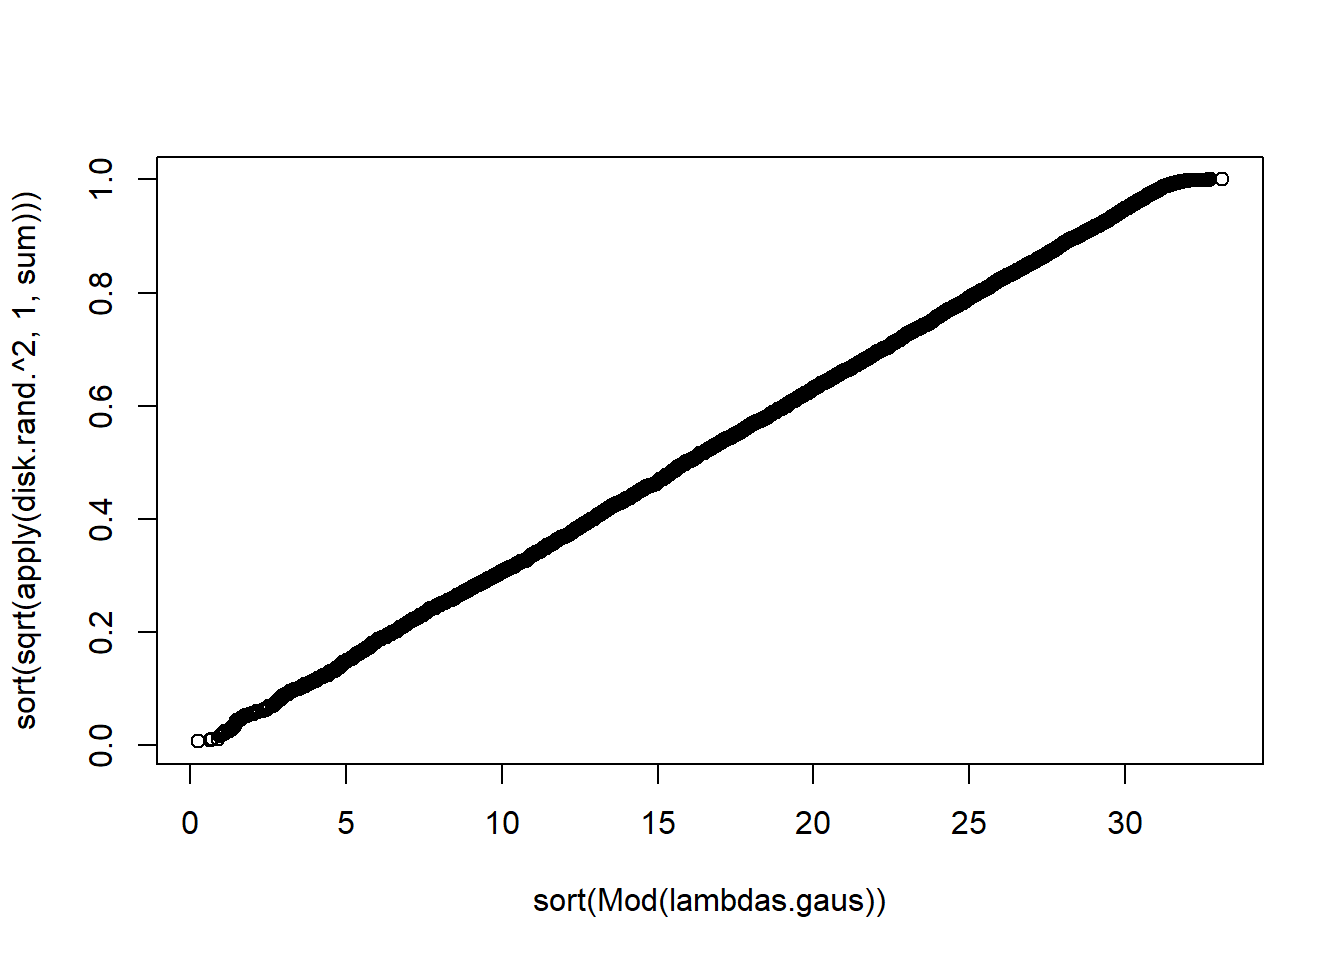
\includegraphics{TriangleRotation_files/figure-latex/unnamed-chunk-7-1.pdf}
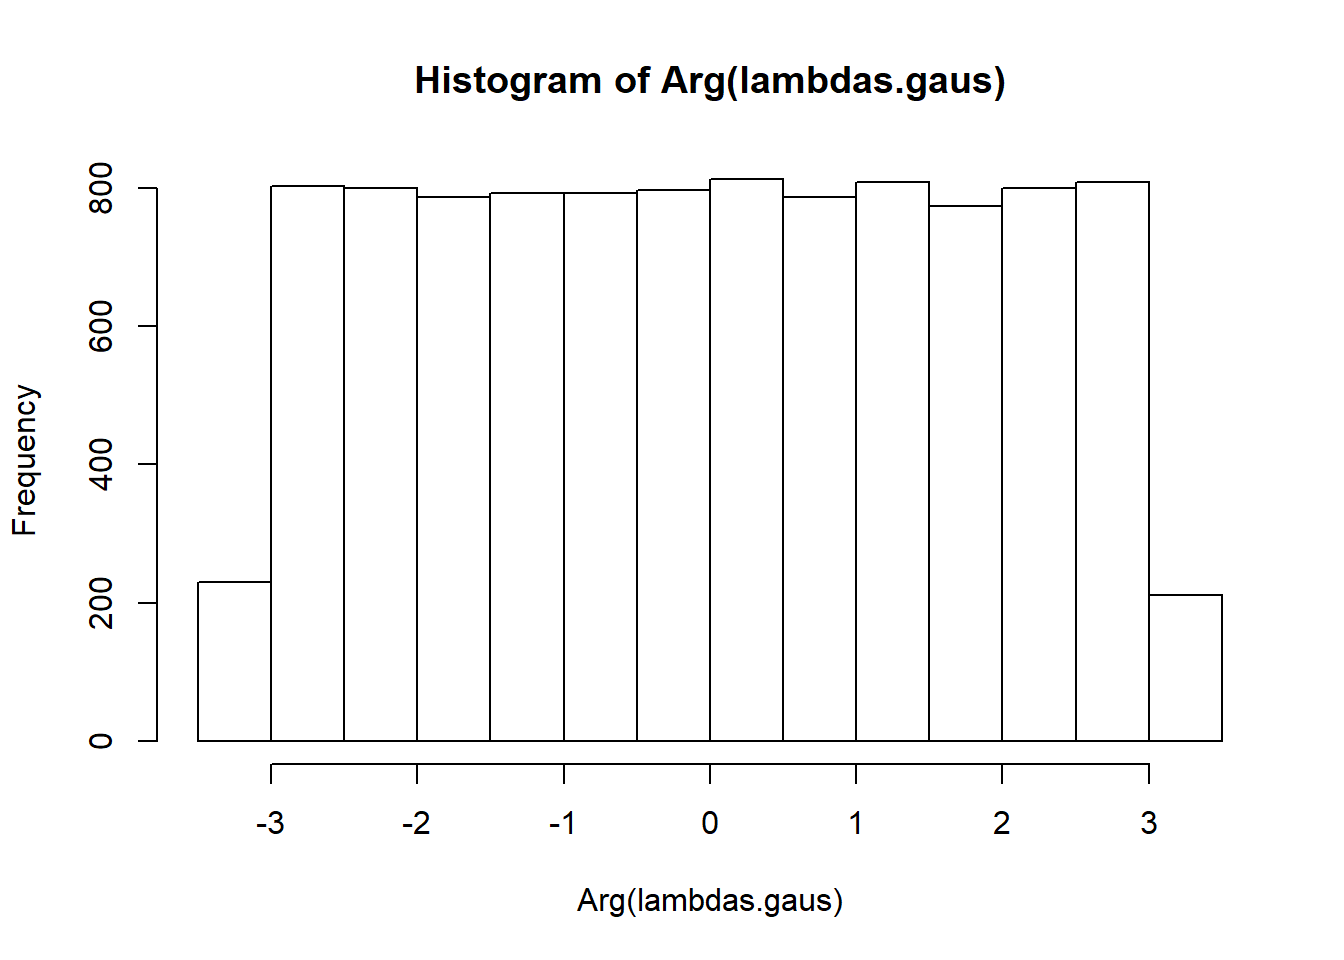
\includegraphics{TriangleRotation_files/figure-latex/unnamed-chunk-7-2.pdf}
\includegraphics{TriangleRotation_files/figure-latex/unnamed-chunk-7-3.pdf}
\includegraphics{TriangleRotation_files/figure-latex/unnamed-chunk-7-4.pdf}
\includegraphics{TriangleRotation_files/figure-latex/unnamed-chunk-7-5.pdf}
\includegraphics{TriangleRotation_files/figure-latex/unnamed-chunk-7-6.pdf}
\includegraphics{TriangleRotation_files/figure-latex/unnamed-chunk-7-7.pdf}
\includegraphics{TriangleRotation_files/figure-latex/unnamed-chunk-7-8.pdf}
\includegraphics{TriangleRotation_files/figure-latex/unnamed-chunk-7-9.pdf}
\includegraphics{TriangleRotation_files/figure-latex/unnamed-chunk-7-10.pdf}
\includegraphics{TriangleRotation_files/figure-latex/unnamed-chunk-7-11.pdf}
\includegraphics{TriangleRotation_files/figure-latex/unnamed-chunk-7-12.pdf}
\includegraphics{TriangleRotation_files/figure-latex/unnamed-chunk-7-13.pdf}
\includegraphics{TriangleRotation_files/figure-latex/unnamed-chunk-7-14.pdf}
\includegraphics{TriangleRotation_files/figure-latex/unnamed-chunk-7-15.pdf}
\includegraphics{TriangleRotation_files/figure-latex/unnamed-chunk-7-16.pdf}
\includegraphics{TriangleRotation_files/figure-latex/unnamed-chunk-7-17.pdf}
\includegraphics{TriangleRotation_files/figure-latex/unnamed-chunk-7-18.pdf}
\includegraphics{TriangleRotation_files/figure-latex/unnamed-chunk-7-19.pdf}
\includegraphics{TriangleRotation_files/figure-latex/unnamed-chunk-7-20.pdf}
\includegraphics{TriangleRotation_files/figure-latex/unnamed-chunk-7-21.pdf}
\includegraphics{TriangleRotation_files/figure-latex/unnamed-chunk-7-22.pdf}
\includegraphics{TriangleRotation_files/figure-latex/unnamed-chunk-7-23.pdf}
\includegraphics{TriangleRotation_files/figure-latex/unnamed-chunk-7-24.pdf}
\includegraphics{TriangleRotation_files/figure-latex/unnamed-chunk-7-25.pdf}
\includegraphics{TriangleRotation_files/figure-latex/unnamed-chunk-7-26.pdf}
\includegraphics{TriangleRotation_files/figure-latex/unnamed-chunk-7-27.pdf}
\includegraphics{TriangleRotation_files/figure-latex/unnamed-chunk-7-28.pdf}
\includegraphics{TriangleRotation_files/figure-latex/unnamed-chunk-7-29.pdf}

三角形の枚数と均等角との関係は次のようになる。

\begin{Shaded}
\begin{Highlighting}[]
\NormalTok{estimated.theta <-}\StringTok{ }\KeywordTok{sapply}\NormalTok{(outs, }\ControlFlowTok{function}\NormalTok{(x)\{}\KeywordTok{return}\NormalTok{(x}\OperatorTok{$}\NormalTok{theta)\})}\OperatorTok{/}\NormalTok{pi}
\KeywordTok{plot}\NormalTok{(ks,estimated.theta,}\DataTypeTok{ylab=}\StringTok{"angle, unit=PI"}\NormalTok{)}
\end{Highlighting}
\end{Shaded}

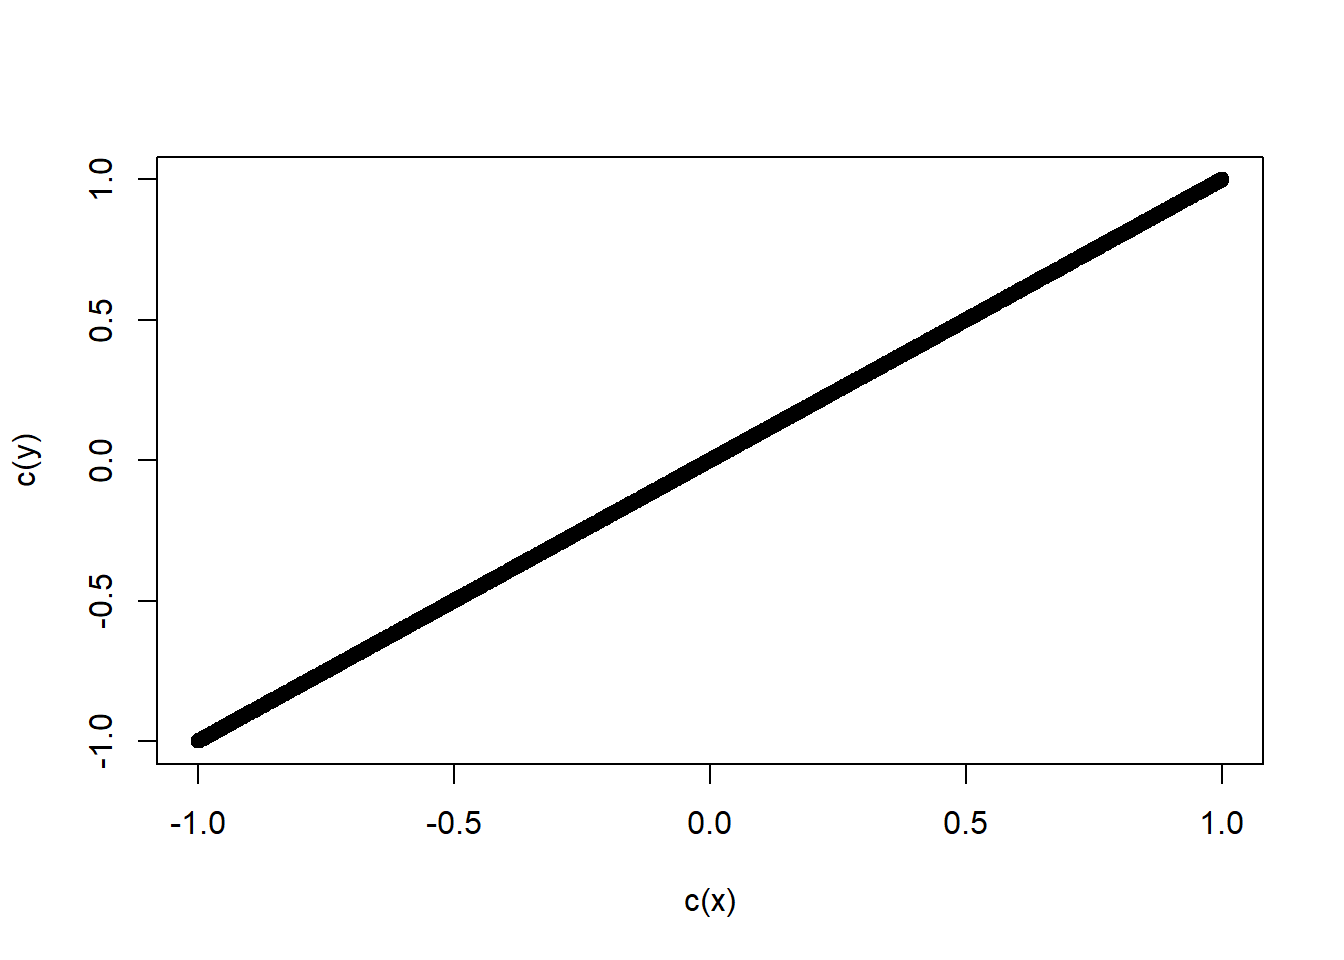
\includegraphics{TriangleRotation_files/figure-latex/unnamed-chunk-8-1.pdf}

\begin{Shaded}
\begin{Highlighting}[]
\CommentTok{#abline(h=c(1,1/2,1/3,1/4))}
\end{Highlighting}
\end{Shaded}

\subsection{三角形の枚数と周回均等角の関係}\label{ux4e09ux89d2ux5f62ux306eux679aux6570ux3068ux5468ux56deux5747ux7b49ux89d2ux306eux95a2ux4fc2}

正三角形の枚数が2、4、8枚の場合を重ねてプロットするとわかるように、枚数の約数の「周回角度」が含まれる。

\begin{Shaded}
\begin{Highlighting}[]
\KeywordTok{matplot}\NormalTok{(}\KeywordTok{cbind}\NormalTok{(outs[[}\DecValTok{1}\NormalTok{]]}\OperatorTok{$}\NormalTok{cosAs,outs[[}\DecValTok{3}\NormalTok{]]}\OperatorTok{$}\NormalTok{cosAs,outs[[}\DecValTok{7}\NormalTok{]]}\OperatorTok{$}\NormalTok{cosAs),}\DataTypeTok{type=}\StringTok{"l"}\NormalTok{) }
\end{Highlighting}
\end{Shaded}

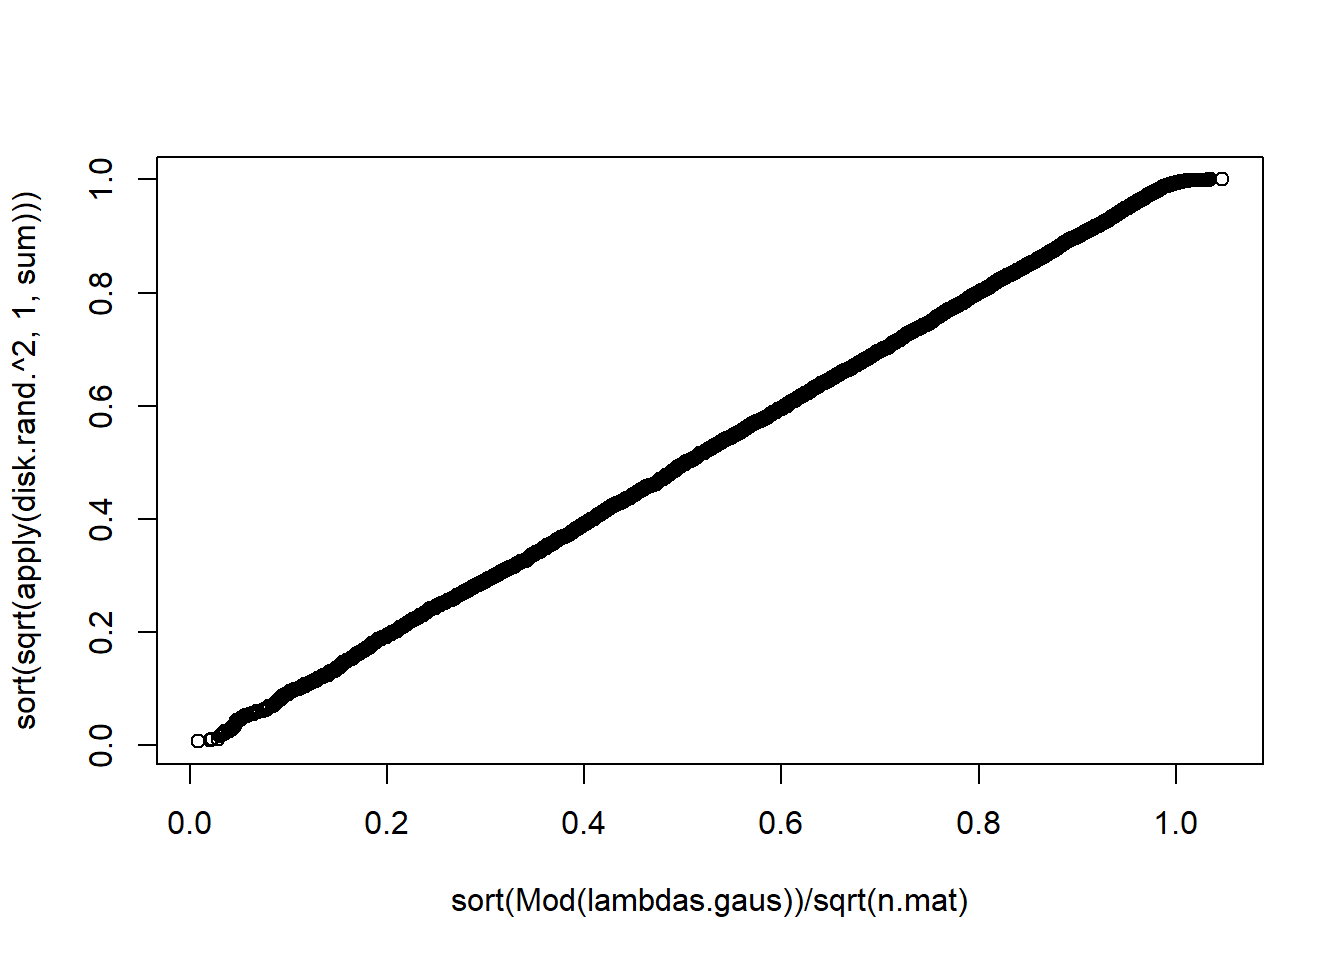
\includegraphics{TriangleRotation_files/figure-latex/unnamed-chunk-9-1.pdf}

2枚、3枚、6枚では?

\begin{Shaded}
\begin{Highlighting}[]
\KeywordTok{matplot}\NormalTok{(}\KeywordTok{cbind}\NormalTok{(outs[[}\DecValTok{1}\NormalTok{]]}\OperatorTok{$}\NormalTok{cosAs,outs[[}\DecValTok{2}\NormalTok{]]}\OperatorTok{$}\NormalTok{cosAs,outs[[}\DecValTok{5}\NormalTok{]]}\OperatorTok{$}\NormalTok{cosAs),}\DataTypeTok{type=}\StringTok{"l"}\NormalTok{) }
\end{Highlighting}
\end{Shaded}

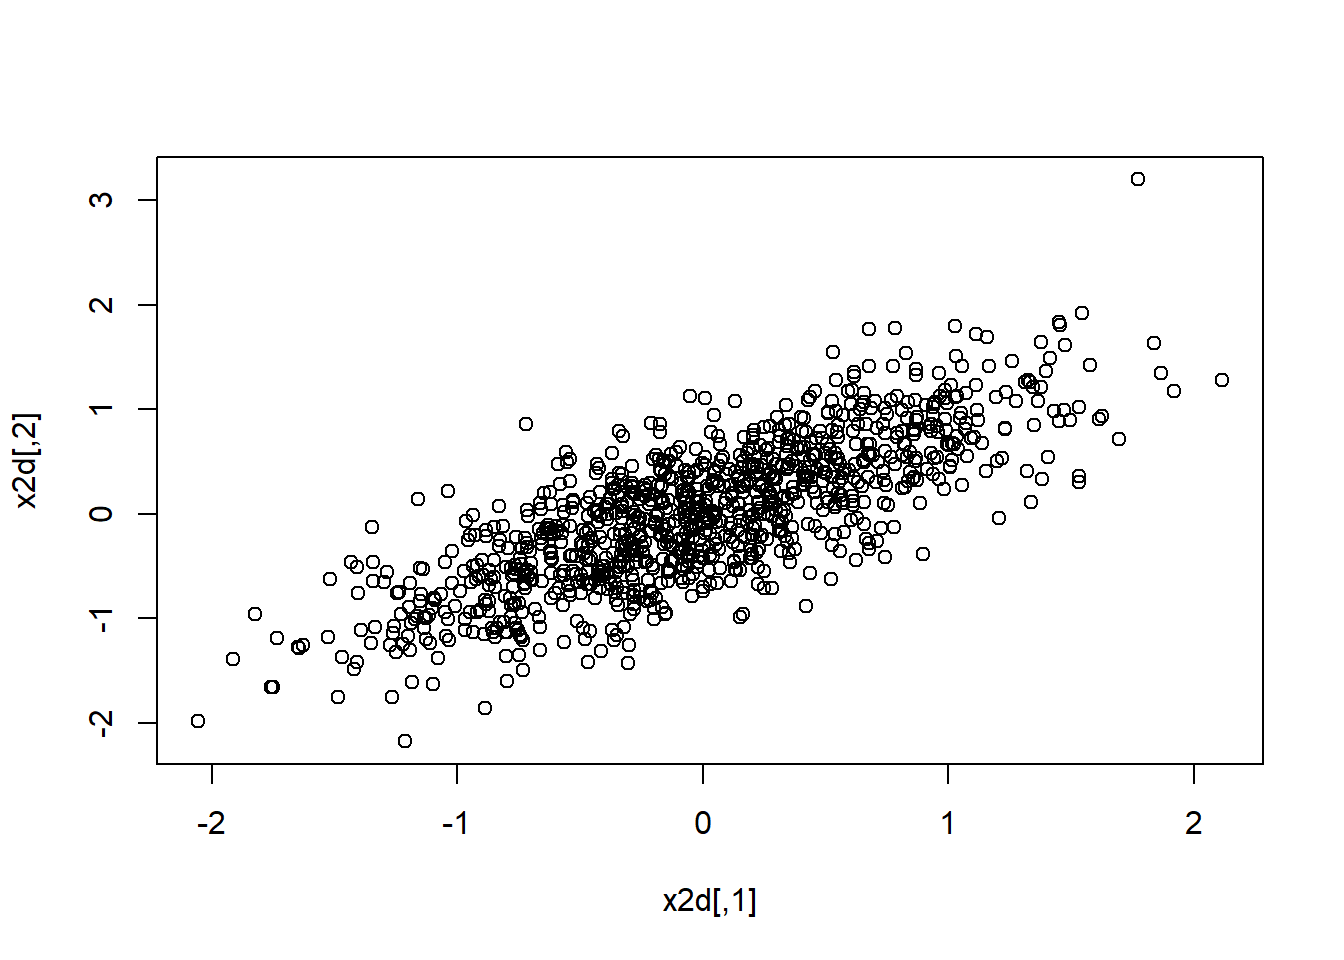
\includegraphics{TriangleRotation_files/figure-latex/unnamed-chunk-10-1.pdf}
5枚、6枚、10枚、30枚では?

\begin{Shaded}
\begin{Highlighting}[]
\KeywordTok{matplot}\NormalTok{(}\KeywordTok{cbind}\NormalTok{(outs[[}\DecValTok{4}\NormalTok{]]}\OperatorTok{$}\NormalTok{cosAs,outs[[}\DecValTok{5}\NormalTok{]]}\OperatorTok{$}\NormalTok{cosAs,outs[[}\DecValTok{9}\NormalTok{]]}\OperatorTok{$}\NormalTok{cosAs,outs[[}\DecValTok{29}\NormalTok{]]}\OperatorTok{$}\NormalTok{cosAs),}\DataTypeTok{type=}\StringTok{"l"}\NormalTok{) }
\end{Highlighting}
\end{Shaded}

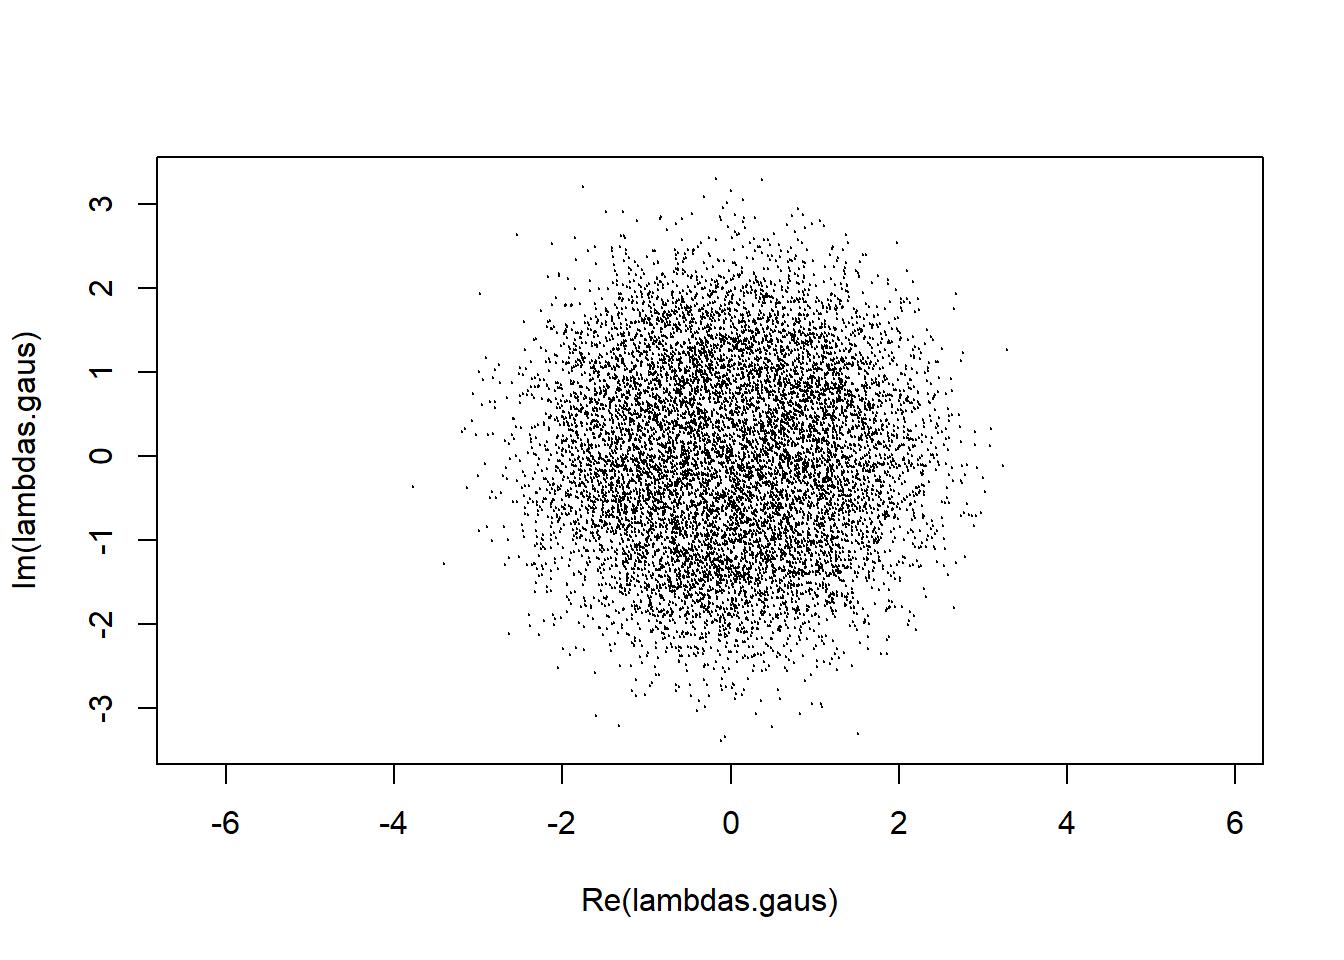
\includegraphics{TriangleRotation_files/figure-latex/unnamed-chunk-11-1.pdf}

この「角度」と枚数とその約数との関係に、ある種の分子分母関係があることがわかる。

\subsection{7枚以上の三角形で閉じる}\label{ux679aux4ee5ux4e0aux306eux4e09ux89d2ux5f62ux3067ux9589ux3058ux308b}

上の例では、7枚以上においても、均等角を算出した。

しかしながら、この角では、三角形同士が交叉することとなり、3次元空間の閉多面体としては不適当である。

したがって、7枚以上の場合には、等角度ではあるが、角度の正負が交互になるような均質性を仮定して、閉じさせることを考える。

実際に、実施してみると、奇数枚の場合には、正負が反転しない場合が発生し、そのような閉じ方が成立しないことがわかる。

\begin{Shaded}
\begin{Highlighting}[]
\NormalTok{ks2 <-}\StringTok{ }\DecValTok{7}\OperatorTok{:}\DecValTok{30}
\NormalTok{outs.alt <-}\StringTok{ }\KeywordTok{list}\NormalTok{()}
\ControlFlowTok{for}\NormalTok{(i }\ControlFlowTok{in} \DecValTok{1}\OperatorTok{:}\KeywordTok{length}\NormalTok{(ks2))\{}
\NormalTok{  outs.alt[[i]] <-}\StringTok{ }\KeywordTok{my.tri.cycle}\NormalTok{(}\DataTypeTok{k=}\NormalTok{ks2[i],}\DataTypeTok{sign.alt=}\OtherTok{TRUE}\NormalTok{) }\CommentTok{# sign.alt=TRUEにより、角の正負を交互にする}
\NormalTok{\}}
\end{Highlighting}
\end{Shaded}

\includegraphics{TriangleRotation_files/figure-latex/unnamed-chunk-12-1.pdf}
\includegraphics{TriangleRotation_files/figure-latex/unnamed-chunk-12-2.pdf}
\includegraphics{TriangleRotation_files/figure-latex/unnamed-chunk-12-3.pdf}
\includegraphics{TriangleRotation_files/figure-latex/unnamed-chunk-12-4.pdf}
\includegraphics{TriangleRotation_files/figure-latex/unnamed-chunk-12-5.pdf}
\includegraphics{TriangleRotation_files/figure-latex/unnamed-chunk-12-6.pdf}
\includegraphics{TriangleRotation_files/figure-latex/unnamed-chunk-12-7.pdf}
\includegraphics{TriangleRotation_files/figure-latex/unnamed-chunk-12-8.pdf}
\includegraphics{TriangleRotation_files/figure-latex/unnamed-chunk-12-9.pdf}
\includegraphics{TriangleRotation_files/figure-latex/unnamed-chunk-12-10.pdf}
\includegraphics{TriangleRotation_files/figure-latex/unnamed-chunk-12-11.pdf}
\includegraphics{TriangleRotation_files/figure-latex/unnamed-chunk-12-12.pdf}
\includegraphics{TriangleRotation_files/figure-latex/unnamed-chunk-12-13.pdf}
\includegraphics{TriangleRotation_files/figure-latex/unnamed-chunk-12-14.pdf}
\includegraphics{TriangleRotation_files/figure-latex/unnamed-chunk-12-15.pdf}
\includegraphics{TriangleRotation_files/figure-latex/unnamed-chunk-12-16.pdf}
\includegraphics{TriangleRotation_files/figure-latex/unnamed-chunk-12-17.pdf}
\includegraphics{TriangleRotation_files/figure-latex/unnamed-chunk-12-18.pdf}
\includegraphics{TriangleRotation_files/figure-latex/unnamed-chunk-12-19.pdf}
\includegraphics{TriangleRotation_files/figure-latex/unnamed-chunk-12-20.pdf}
\includegraphics{TriangleRotation_files/figure-latex/unnamed-chunk-12-21.pdf}
\includegraphics{TriangleRotation_files/figure-latex/unnamed-chunk-12-22.pdf}
\includegraphics{TriangleRotation_files/figure-latex/unnamed-chunk-12-23.pdf}
\includegraphics{TriangleRotation_files/figure-latex/unnamed-chunk-12-24.pdf}

算出された角を、上段に偶数枚の場合、下段に奇数枚の場合を書くと、偶数枚の場合には値がありるが、奇数枚の場合には、値が得られないことがわかる。

\begin{Shaded}
\begin{Highlighting}[]
\NormalTok{outs.alt.ang <-}\StringTok{ }\KeywordTok{sapply}\NormalTok{(outs.alt,}\ControlFlowTok{function}\NormalTok{(x)\{}\KeywordTok{return}\NormalTok{(x}\OperatorTok{$}\NormalTok{theta)\})}
\KeywordTok{matrix}\NormalTok{(outs.alt.ang,}\DataTypeTok{nrow=}\DecValTok{2}\NormalTok{)}
\end{Highlighting}
\end{Shaded}

\begin{verbatim}
##          [,1]     [,2] [,3]     [,4]     [,5] [,6]      [,7]     [,8] [,9]
## [1,]       NA       NA   NA       NA       NA   NA        NA       NA   NA
## [2,] 1.385812 1.805945    0 1.034656 1.392083    0 0.8590782 1.178881    0
##          [,10]    [,11] [,12]
## [1,]        NA       NA    NA
## [2,] 0.7524773 1.040927     0
\end{verbatim}

\begin{Shaded}
\begin{Highlighting}[]
\KeywordTok{plot}\NormalTok{(}\KeywordTok{matrix}\NormalTok{(ks2,}\DataTypeTok{nrow=}\DecValTok{2}\NormalTok{)[}\DecValTok{2}\NormalTok{,],}\KeywordTok{matrix}\NormalTok{(outs.alt.ang,}\DataTypeTok{nrow=}\DecValTok{2}\NormalTok{)[}\DecValTok{2}\NormalTok{,])}
\end{Highlighting}
\end{Shaded}

\includegraphics{TriangleRotation_files/figure-latex/unnamed-chunk-13-1.pdf}

角度の符号反転の場合には、枚数の約数関係に、反転無しの場合のような規則は存在しないようである。

以下に、8枚、16枚の関係を示す。

\begin{Shaded}
\begin{Highlighting}[]
\KeywordTok{matplot}\NormalTok{(}\KeywordTok{cbind}\NormalTok{(outs.alt[[}\DecValTok{2}\NormalTok{]]}\OperatorTok{$}\NormalTok{cosAs,outs.alt[[}\DecValTok{10}\NormalTok{]]}\OperatorTok{$}\NormalTok{cosAs),}\DataTypeTok{type=}\StringTok{"l"}\NormalTok{) }
\end{Highlighting}
\end{Shaded}

\includegraphics{TriangleRotation_files/figure-latex/unnamed-chunk-14-1.pdf}

\subsection{幾何学的に角を求める}\label{ux5e7eux4f55ux5b66ux7684ux306bux89d2ux3092ux6c42ux3081ux308b}

正三角形を1点を中心にk枚貼り合わせて、元に戻るようにする。

ただし、k = 6t + s の時には、s = 0
ならば、\(2 \times t \times \pi\)の角をk等分することとし、s =
1,2,\ldots{},5ならば、\(2 \times (t+1) \times \pi\)
の角をk等分することとする。

計算してみる。

\begin{itemize}
\tightlist
\item
  \(2 t \pi\)をk等分して閉じるとき、連結する三角形のなす角\(\theta\)は
\end{itemize}

\[
\phi = \frac{2 t \pi}{k}\\ 
L = \frac{1}{2 \sin{\frac{\phi}{2}}\\
\cos{\theta} = \frac{4}{3} * (\frac{1}{2 L^2} - \frac{5}{4})
\]

関数にする。

\begin{Shaded}
\begin{Highlighting}[]
\CommentTok{# k は三角形の枚数}
\NormalTok{my.tri.angle <-}\StringTok{ }\ControlFlowTok{function}\NormalTok{(k)\{}
  \CommentTok{# k = t * 6 の時は、角度0}
  \CommentTok{# k = t * 6 + s (s<6) の時は、2 pi * (t+1) の角をk等分する}
\NormalTok{  six.info <-}\StringTok{ }\NormalTok{(k}\OperatorTok{-}\DecValTok{1}\NormalTok{)}\OperatorTok\DecValTok{6}
  \CommentTok{# six.info + 1 周させる}
  \CommentTok{# 1つの三角形が稼ぐべき、二次元平面的な角度}
\NormalTok{  phi <-}\StringTok{ }\DecValTok{2} \OperatorTok{*}\StringTok{ }\NormalTok{pi }\OperatorTok{*}\StringTok{ }\NormalTok{(six.info }\OperatorTok{+}\StringTok{ }\DecValTok{1}\NormalTok{) }\OperatorTok{/}\StringTok{ }\NormalTok{k}
  \CommentTok{# 中心頂点から見下ろした時に、正三角形の周辺頂点の原点からの距離(2D平面上の距離)}
\NormalTok{  L <-}\StringTok{ }\DecValTok{1}\OperatorTok{/}\NormalTok{(}\DecValTok{2}\OperatorTok{*}\KeywordTok{sin}\NormalTok{(phi}\OperatorTok{/}\DecValTok{2}\NormalTok{))}
  \CommentTok{# 幾何的な関係を色々やると、正三角形の周辺頂点を一つ飛ばしにした2頂点と}
  \CommentTok{# その間にある周辺頂点と中心頂点の中点とをそれぞれ結び、その2つの線分ベクトルのcos(theta)を計算すると以下の式となる}
\NormalTok{  costheta <-}\StringTok{ }\DecValTok{4}\OperatorTok{/}\DecValTok{3} \OperatorTok{*}\StringTok{ }\NormalTok{(}\DecValTok{1}\OperatorTok{/}\NormalTok{(}\DecValTok{2}\OperatorTok{*}\NormalTok{L}\OperatorTok{^}\DecValTok{2}\NormalTok{) }\OperatorTok{-}\StringTok{ }\DecValTok{5}\OperatorTok{/}\DecValTok{4}\NormalTok{)}
  \CommentTok{# 計算誤差のためにちょっと工夫をして}
  \ControlFlowTok{if}\NormalTok{(costheta }\OperatorTok{>}\StringTok{ }\DecValTok{1}\NormalTok{) costheta <-}\StringTok{ }\DecValTok{1}
  \ControlFlowTok{if}\NormalTok{(costheta }\OperatorTok{<}\StringTok{ }\OperatorTok{-}\DecValTok{1}\NormalTok{) costheta <-}\StringTok{ }\OperatorTok{-}\DecValTok{1}
\NormalTok{  theta <-}\StringTok{ }\KeywordTok{acos}\NormalTok{(costheta)}
  \CommentTok{# 最終的に、2つの三角形のなす角を、pi-thetaとして返す}
  \KeywordTok{return}\NormalTok{(pi }\OperatorTok{-}\StringTok{ }\NormalTok{theta)}
\NormalTok{\}}
\end{Highlighting}
\end{Shaded}

多数の角を評価して推定した結果と一致することを確かめる。

\begin{Shaded}
\begin{Highlighting}[]
\CommentTok{# ks <- 2:30}
\NormalTok{t <-}\StringTok{ }\KeywordTok{rep}\NormalTok{(}\DecValTok{0}\NormalTok{,}\KeywordTok{length}\NormalTok{(ks))}
\ControlFlowTok{for}\NormalTok{(i }\ControlFlowTok{in} \DecValTok{1}\OperatorTok{:}\KeywordTok{length}\NormalTok{(ks))\{}
\NormalTok{  t[i] <-}\StringTok{ }\KeywordTok{my.tri.angle}\NormalTok{(ks[i])}
\NormalTok{\}}
\KeywordTok{plot}\NormalTok{(t)}
\end{Highlighting}
\end{Shaded}

\includegraphics{TriangleRotation_files/figure-latex/unnamed-chunk-16-1.pdf}

\begin{Shaded}
\begin{Highlighting}[]
\KeywordTok{plot}\NormalTok{(estimated.theta, t}\OperatorTok{/}\NormalTok{pi)}
\KeywordTok{abline}\NormalTok{(}\DecValTok{0}\NormalTok{,}\DecValTok{1}\NormalTok{,}\DataTypeTok{col=}\DecValTok{2}\NormalTok{)}
\end{Highlighting}
\end{Shaded}

\includegraphics{TriangleRotation_files/figure-latex/unnamed-chunk-17-1.pdf}

\subsection{偶数個のk \textgreater{}
6について、角度を正負交互にして1周する場合の幾何的な解}\label{ux5076ux6570ux500bux306ek-6ux306bux3064ux3044ux3066ux89d2ux5ea6ux3092ux6b63ux8ca0ux4ea4ux4e92ux306bux3057ux3066ux5468ux3059ux308bux5834ux5408ux306eux5e7eux4f55ux7684ux306aux89e3}

\(k = 2p\)枚の正三角形を用いる。

外周頂点のz座標は絶対値は等しく、正負が交互になるから、ある2枚の正三角形は、原点(0,0,0)を中心として、

(x,-y,-z), (x',0,z),(x,y,-z)の3点となる。

こららが満足する条件は \[
x^2 + y^2 + z^2 = x^2 + (-y)^2 + (-z)^2 = x^2 + y^2 + (-z)^2 = 1\\
x'^2 + z^2 = 1\\
(x-x')^2 + (-y)^2 + (2z)^2 = 1\\
\]
また、外周辺の中点のz座標は0であり、隣り合う、中心と外周辺中点を結ぶベクトルとのなす角は、\(\frac{2\pi}{k}\)である。

中点2つは\((\frac{x+x'}{2},-\frac{y}{2},0),(\frac{x+x'}{2},\frac{y}{2},0)\)であるから
\[
\frac{(\frac{x+x'}{2})^2 - (\frac{y}{2})^2}{(\frac{x+x'}{2})^2 + (\frac{y}{2})^2} = \cos{\frac{2\pi}{k}}
\] これらを解くと \[
x' = \sqrt{\frac{3}{2}\frac{1}{1+\cos{\frac{2\pi}{k}}}}\\
z = \sqrt{1-x'^2}\\
x = x' \cos{\frac{2\pi}{k}}\\
y = x' \sqrt{(1+\cos{\frac{2\pi}{k}})(1-\cos{\frac{2\pi}{k}})}
\] 2枚の三角形がなす角\(\theta\)は (x-x'/2,-y,-3/2z)
と(x-x'/2,y,-3/2z)とがなす角の外角であるから、

\[
\cos{(\pi-\theta)} = \frac{(x-\frac{x'}{2})^2-y^2+9/4z^2}{(x-\frac{x'}{2})^2+y^2+9/4z^2}
\]

これを関数にして

\begin{Shaded}
\begin{Highlighting}[]
\NormalTok{my.updown.ang <-}\StringTok{ }\ControlFlowTok{function}\NormalTok{(k)\{}
\NormalTok{  C <-}\StringTok{ }\KeywordTok{cos}\NormalTok{(}\DecValTok{2}\OperatorTok{*}\NormalTok{pi}\OperatorTok{/}\NormalTok{k)}
\NormalTok{  x. <-}\StringTok{ }\KeywordTok{sqrt}\NormalTok{(}\DecValTok{3}\OperatorTok{/}\NormalTok{(}\DecValTok{2} \OperatorTok{*}\StringTok{ }\NormalTok{(}\DecValTok{1}\OperatorTok{+}\NormalTok{C)))}
\NormalTok{  z <-}\StringTok{ }\KeywordTok{sqrt}\NormalTok{(}\DecValTok{1}\OperatorTok{-}\NormalTok{x.}\OperatorTok{^}\DecValTok{2}\NormalTok{)}
\NormalTok{  x <-}\StringTok{ }\NormalTok{x. }\OperatorTok{*}\StringTok{ }\NormalTok{C}
\NormalTok{  y <-}\StringTok{ }\NormalTok{x. }\OperatorTok{*}\StringTok{ }\KeywordTok{sqrt}\NormalTok{((}\DecValTok{1}\OperatorTok{+}\NormalTok{C)}\OperatorTok{*}\NormalTok{(}\DecValTok{1}\OperatorTok{-}\NormalTok{C))}
\NormalTok{  tmp.cos <-}\StringTok{ }\NormalTok{((x}\OperatorTok{-}\NormalTok{x.}\OperatorTok{/}\DecValTok{2}\NormalTok{)}\OperatorTok{^}\DecValTok{2} \OperatorTok{-}\StringTok{ }\NormalTok{y}\OperatorTok{^}\DecValTok{2} \OperatorTok{+}\StringTok{ }\DecValTok{9}\OperatorTok{/}\DecValTok{4}\OperatorTok{*}\NormalTok{z}\OperatorTok{^}\DecValTok{2}\NormalTok{)}\OperatorTok{/}\NormalTok{((x}\OperatorTok{-}\NormalTok{x.}\OperatorTok{/}\DecValTok{2}\NormalTok{)}\OperatorTok{^}\DecValTok{2} \OperatorTok{+}\StringTok{ }\NormalTok{y}\OperatorTok{^}\DecValTok{2} \OperatorTok{+}\StringTok{ }\DecValTok{9}\OperatorTok{/}\DecValTok{4}\OperatorTok{*}\NormalTok{z}\OperatorTok{^}\DecValTok{2}\NormalTok{)}
\NormalTok{  theta <-}\StringTok{ }\NormalTok{pi }\OperatorTok{-}\StringTok{ }\KeywordTok{acos}\NormalTok{(tmp.cos)}
  \KeywordTok{return}\NormalTok{(theta) }
\NormalTok{\}}
\end{Highlighting}
\end{Shaded}

\begin{Shaded}
\begin{Highlighting}[]
\NormalTok{out.alt.}\DecValTok{2}\NormalTok{ <-}\StringTok{ }\KeywordTok{rep}\NormalTok{(}\DecValTok{0}\NormalTok{,}\KeywordTok{length}\NormalTok{(ks2))}
\ControlFlowTok{for}\NormalTok{(i }\ControlFlowTok{in} \DecValTok{1}\OperatorTok{:}\KeywordTok{length}\NormalTok{(ks2))\{}
\NormalTok{  out.alt.}\DecValTok{2}\NormalTok{[i] <-}\StringTok{ }\KeywordTok{my.updown.ang}\NormalTok{(ks2[i])}
\NormalTok{\}}

\KeywordTok{plot}\NormalTok{(ks2,out.alt.}\DecValTok{2}\NormalTok{)}
\end{Highlighting}
\end{Shaded}

\includegraphics{TriangleRotation_files/figure-latex/unnamed-chunk-19-1.pdf}

角度をパラメタ化して探索した場合は、2周以上しても良いので、なるべく小さい角で元に戻る値を求めているため、幾何的算出結果と合致しない。

\begin{Shaded}
\begin{Highlighting}[]
\NormalTok{outs.alt.ang}
\end{Highlighting}
\end{Shaded}

\begin{verbatim}
##  [1]        NA 1.3858123        NA 1.8059455        NA 0.0000000        NA
##  [8] 1.0346563        NA 1.3920830        NA 0.0000000        NA 0.8590782
## [15]        NA 1.1788811        NA 0.0000000        NA 0.7524773        NA
## [22] 1.0409269        NA 0.0000000
\end{verbatim}

\begin{Shaded}
\begin{Highlighting}[]
\NormalTok{out.alt.}\DecValTok{2}
\end{Highlighting}
\end{Shaded}

\begin{verbatim}
##  [1] 1.040208 1.398370 1.635018 1.809114 1.944444 2.053416 2.143402 2.219151
##  [9] 2.283897 2.339937 2.388956 2.432220 2.470703 2.505168 2.536222 2.564352
## [17] 2.589958 2.613368 2.634855 2.654649 2.672944 2.689905 2.705673 2.720372
\end{verbatim}

枚数が偶数の場合について、悉皆探索最小角と、幾何的産出角の関係を示す。

\begin{Shaded}
\begin{Highlighting}[]
\KeywordTok{plot}\NormalTok{(}\KeywordTok{matrix}\NormalTok{(outs.alt.ang,}\DataTypeTok{nrow=}\DecValTok{2}\NormalTok{)[}\DecValTok{2}\NormalTok{,],}\KeywordTok{matrix}\NormalTok{(out.alt.}\DecValTok{2}\NormalTok{,}\DataTypeTok{nrow=}\DecValTok{2}\NormalTok{)[}\DecValTok{2}\NormalTok{,])}
\end{Highlighting}
\end{Shaded}

\includegraphics{TriangleRotation_files/figure-latex/unnamed-chunk-21-1.pdf}

合致関係は、以下のようなグラフとして表示するとわかりやすい。

また、奇数枚の場合がなぜ不適当かも、視覚的に表現されている。

\begin{Shaded}
\begin{Highlighting}[]
\ControlFlowTok{for}\NormalTok{(i }\ControlFlowTok{in} \DecValTok{1}\OperatorTok{:}\KeywordTok{length}\NormalTok{(ks2))\{}
\NormalTok{  tmp <-}\StringTok{ }\KeywordTok{cbind}\NormalTok{(outs.alt[[i]]}\OperatorTok{$}\NormalTok{cosAs,outs.alt[[i]]}\OperatorTok{$}\NormalTok{cosNs)}
  \KeywordTok{matplot}\NormalTok{(outs.alt[[i]]}\OperatorTok{$}\NormalTok{theta.list}\OperatorTok{/}\NormalTok{pi,tmp,}\DataTypeTok{type=}\StringTok{"l"}\NormalTok{)}
  \KeywordTok{abline}\NormalTok{(}\DataTypeTok{v =}\NormalTok{ out.alt.}\DecValTok{2}\NormalTok{[i]}\OperatorTok{/}\NormalTok{pi,}\DataTypeTok{col=}\DecValTok{4}\NormalTok{)}
\NormalTok{\}}
\end{Highlighting}
\end{Shaded}

\includegraphics{TriangleRotation_files/figure-latex/unnamed-chunk-22-1.pdf}
\includegraphics{TriangleRotation_files/figure-latex/unnamed-chunk-22-2.pdf}
\includegraphics{TriangleRotation_files/figure-latex/unnamed-chunk-22-3.pdf}
\includegraphics{TriangleRotation_files/figure-latex/unnamed-chunk-22-4.pdf}
\includegraphics{TriangleRotation_files/figure-latex/unnamed-chunk-22-5.pdf}
\includegraphics{TriangleRotation_files/figure-latex/unnamed-chunk-22-6.pdf}
\includegraphics{TriangleRotation_files/figure-latex/unnamed-chunk-22-7.pdf}
\includegraphics{TriangleRotation_files/figure-latex/unnamed-chunk-22-8.pdf}
\includegraphics{TriangleRotation_files/figure-latex/unnamed-chunk-22-9.pdf}
\includegraphics{TriangleRotation_files/figure-latex/unnamed-chunk-22-10.pdf}
\includegraphics{TriangleRotation_files/figure-latex/unnamed-chunk-22-11.pdf}
\includegraphics{TriangleRotation_files/figure-latex/unnamed-chunk-22-12.pdf}
\includegraphics{TriangleRotation_files/figure-latex/unnamed-chunk-22-13.pdf}
\includegraphics{TriangleRotation_files/figure-latex/unnamed-chunk-22-14.pdf}
\includegraphics{TriangleRotation_files/figure-latex/unnamed-chunk-22-15.pdf}
\includegraphics{TriangleRotation_files/figure-latex/unnamed-chunk-22-16.pdf}
\includegraphics{TriangleRotation_files/figure-latex/unnamed-chunk-22-17.pdf}
\includegraphics{TriangleRotation_files/figure-latex/unnamed-chunk-22-18.pdf}
\includegraphics{TriangleRotation_files/figure-latex/unnamed-chunk-22-19.pdf}
\includegraphics{TriangleRotation_files/figure-latex/unnamed-chunk-22-20.pdf}
\includegraphics{TriangleRotation_files/figure-latex/unnamed-chunk-22-21.pdf}
\includegraphics{TriangleRotation_files/figure-latex/unnamed-chunk-22-22.pdf}
\includegraphics{TriangleRotation_files/figure-latex/unnamed-chunk-22-23.pdf}
\includegraphics{TriangleRotation_files/figure-latex/unnamed-chunk-22-24.pdf}

\subsection{必ずしも均等角でないが、閉じるための角度条件}\label{ux5fc5ux305aux3057ux3082ux5747ux7b49ux89d2ux3067ux306aux3044ux304cux9589ux3058ux308bux305fux3081ux306eux89d2ux5ea6ux6761ux4ef6}

今、k枚の正三角形が、 \[
(\theta_1,\theta_2,...,\theta_k)
\] で閉じているとする。

k-1枚目とk枚目との間に2枚を\(\pi\)でピタリと押しつぶした状態で割り込ませ、k+2枚にすることができる。
その時にできる、長さk+2の角度列は

\[
(\theta_1,...,\theta_{k-1},-\pi + \phi, \pi, \theta_k - \phi)
\]

5枚で均等曲げを実行してみる。

\begin{Shaded}
\begin{Highlighting}[]
\NormalTok{k <-}\StringTok{ }\DecValTok{5}
\NormalTok{theta.k <-}\StringTok{ }\NormalTok{t[k}\OperatorTok{-}\DecValTok{1}\NormalTok{]}
\NormalTok{thetas <-}\StringTok{ }\KeywordTok{rep}\NormalTok{(theta.k,k)}

\NormalTok{outk <-}\StringTok{ }\KeywordTok{my.function.tri.rot.series}\NormalTok{(}\DataTypeTok{thetas=}\NormalTok{thetas)}
\KeywordTok{range}\NormalTok{(outk}\OperatorTok{$}\NormalTok{As[}\DecValTok{1}\NormalTok{,] }\OperatorTok{-}\NormalTok{outk}\OperatorTok{$}\NormalTok{As[k}\OperatorTok{+}\DecValTok{1}\NormalTok{,])}
\end{Highlighting}
\end{Shaded}

\begin{verbatim}
## [1] -2.867186e-16 -1.110223e-16
\end{verbatim}

\begin{Shaded}
\begin{Highlighting}[]
\KeywordTok{range}\NormalTok{(outk}\OperatorTok{$}\NormalTok{Ns[}\DecValTok{1}\NormalTok{,] }\OperatorTok{-}\NormalTok{outk}\OperatorTok{$}\NormalTok{Ns[k}\OperatorTok{+}\DecValTok{1}\NormalTok{,])}
\end{Highlighting}
\end{Shaded}

\begin{verbatim}
## [1] 0.000000e+00 2.220446e-16
\end{verbatim}

\begin{Shaded}
\begin{Highlighting}[]
\NormalTok{my.insert.two.tris <-}\StringTok{ }\ControlFlowTok{function}\NormalTok{(theta,}\DataTypeTok{phi =} \FloatTok{0.1}\NormalTok{)\{}
\NormalTok{  k <-}\StringTok{ }\KeywordTok{length}\NormalTok{(theta)}
\NormalTok{  ret <-}\StringTok{ }\KeywordTok{c}\NormalTok{(theta[}\DecValTok{1}\OperatorTok{:}\NormalTok{(k}\OperatorTok{-}\DecValTok{1}\NormalTok{)],}\OperatorTok{-}\NormalTok{pi }\OperatorTok{+}\StringTok{ }\NormalTok{phi,pi,theta[k]}\OperatorTok{-}\NormalTok{phi)}
  \KeywordTok{return}\NormalTok{(ret)}
\NormalTok{\}}
\NormalTok{thetas2 <-}\StringTok{ }\KeywordTok{my.insert.two.tris}\NormalTok{(thetas)}
\NormalTok{k2 <-}\StringTok{ }\KeywordTok{length}\NormalTok{(thetas2)}
\NormalTok{outk2 <-}\StringTok{ }\KeywordTok{my.function.tri.rot.series}\NormalTok{(}\DataTypeTok{thetas=}\NormalTok{thetas2)}
\KeywordTok{range}\NormalTok{(outk2}\OperatorTok{$}\NormalTok{As[}\DecValTok{1}\NormalTok{,] }\OperatorTok{-}\NormalTok{outk2}\OperatorTok{$}\NormalTok{As[k2}\OperatorTok{+}\DecValTok{1}\NormalTok{,])}
\end{Highlighting}
\end{Shaded}

\begin{verbatim}
## [1] -4.86452e-16  0.00000e+00
\end{verbatim}

\begin{Shaded}
\begin{Highlighting}[]
\KeywordTok{range}\NormalTok{(outk2}\OperatorTok{$}\NormalTok{Ns[}\DecValTok{1}\NormalTok{,] }\OperatorTok{-}\NormalTok{outk2}\OperatorTok{$}\NormalTok{Ns[k2}\OperatorTok{+}\DecValTok{1}\NormalTok{,])}
\end{Highlighting}
\end{Shaded}

\begin{verbatim}
## [1] -6.661338e-16  3.330669e-16
\end{verbatim}

2枚貼り合わせ三角形を挿入して角度ベクトルを不均一にした。それを改変して、閉じる・閉じない条件がどうなるか・・・

角度の順序を入れ替えると、閉じなくなる。。。。単純ではない。そりゃそうか。

\begin{Shaded}
\begin{Highlighting}[]
\NormalTok{thetas2.shuffle <-}\StringTok{ }\KeywordTok{sample}\NormalTok{(thetas2)}

\NormalTok{outk3 <-}\StringTok{ }\KeywordTok{my.function.tri.rot.series}\NormalTok{(}\DataTypeTok{thetas=}\NormalTok{thetas2.shuffle)}
\KeywordTok{range}\NormalTok{(outk3}\OperatorTok{$}\NormalTok{As[}\DecValTok{1}\NormalTok{,] }\OperatorTok{-}\NormalTok{outk3}\OperatorTok{$}\NormalTok{As[k2}\OperatorTok{+}\DecValTok{1}\NormalTok{,])}
\end{Highlighting}
\end{Shaded}

\begin{verbatim}
## [1] -0.6884792  1.5669452
\end{verbatim}

\begin{Shaded}
\begin{Highlighting}[]
\KeywordTok{range}\NormalTok{(outk3}\OperatorTok{$}\NormalTok{Ns[}\DecValTok{1}\NormalTok{,] }\OperatorTok{-}\NormalTok{outk3}\OperatorTok{$}\NormalTok{Ns[k2}\OperatorTok{+}\DecValTok{1}\NormalTok{,])}
\end{Highlighting}
\end{Shaded}

\begin{verbatim}
## [1] -0.8769081  1.4592376
\end{verbatim}

\subsection{ジグザグ路が閉じること}\label{ux30b8ux30b0ux30b6ux30b0ux8defux304cux9589ux3058ux308bux3053ux3068}

1頂点周りにk枚の正三角形が並んで閉じる例を検討してきた。

今度は、正三角形がジグザグ路・擬直線周回路をなす場合について検討する。

すでに作成した関数の一部改変で可能である。

4枚で一周する時は、正四面体様の形になるので、3枚を1頂点周りにとった場合と同じ角度で閉じることに注意する。

6枚の場合に\(\pi\)でも辺ベクトルと法線ベクトルとが一致するが、ベクトルの向きとしてそのようになるだけであって、閉じるわけではないことに注意する。

\begin{Shaded}
\begin{Highlighting}[]
\NormalTok{my.tri.zigzag.cycle <-}\StringTok{ }\ControlFlowTok{function}\NormalTok{(k, }\DataTypeTok{s=}\DecValTok{3}\NormalTok{,}\DataTypeTok{numtheta =} \DecValTok{1003}\NormalTok{,}\DataTypeTok{max.theta =} \DecValTok{2} \OperatorTok{*}\StringTok{ }\NormalTok{pi }\OperatorTok{*}\StringTok{ }\DecValTok{1}\NormalTok{,}\DataTypeTok{sign.alt=}\OtherTok{FALSE}\NormalTok{)\{}
\NormalTok{  theta.list <-}\StringTok{ }\KeywordTok{seq}\NormalTok{(}\DataTypeTok{from=}\DecValTok{0}\NormalTok{,}\DataTypeTok{to=}\NormalTok{max.theta,}\DataTypeTok{length=}\NormalTok{numtheta)}
  
\NormalTok{  cosAs <-}\StringTok{ }\NormalTok{cosNs <-}\StringTok{ }\KeywordTok{rep}\NormalTok{(}\DecValTok{0}\NormalTok{,}\KeywordTok{length}\NormalTok{(theta.list))}
\NormalTok{  cosANs.sq <-}\StringTok{ }\NormalTok{cosAs}
  \ControlFlowTok{for}\NormalTok{(ii }\ControlFlowTok{in} \DecValTok{1}\OperatorTok{:}\KeywordTok{length}\NormalTok{(theta.list))\{}
\NormalTok{    thetas <-}\StringTok{ }\KeywordTok{rep}\NormalTok{(theta.list[ii],k)}
    \ControlFlowTok{if}\NormalTok{(sign.alt)\{}
\NormalTok{      thetas <-}\StringTok{ }\NormalTok{thetas }\OperatorTok{*}\StringTok{ }\NormalTok{(}\OperatorTok{-}\DecValTok{1}\NormalTok{)}\OperatorTok{^}\NormalTok{(}\DecValTok{1}\OperatorTok{:}\KeywordTok{length}\NormalTok{(thetas)) }\OperatorTok{*}\StringTok{ }\NormalTok{(}\OperatorTok{-}\DecValTok{1}\NormalTok{)}
\NormalTok{    \}}
\NormalTok{    ANs <-}\StringTok{ }\KeywordTok{list}\NormalTok{()}
\NormalTok{    ANs[[}\DecValTok{1}\NormalTok{]] <-}\StringTok{ }\KeywordTok{list}\NormalTok{(}\DataTypeTok{A=}\NormalTok{A1,}\DataTypeTok{N=}\NormalTok{N1)}
    \ControlFlowTok{for}\NormalTok{(i }\ControlFlowTok{in} \DecValTok{1}\OperatorTok{:}\NormalTok{k)\{}
      \ControlFlowTok{if}\NormalTok{(i }\OperatorTok\StringTok{ }\DecValTok{2} \OperatorTok{==}\StringTok{ }\DecValTok{0}\NormalTok{)\{}
\NormalTok{        tmp <-}\StringTok{ }\KeywordTok{my.function.tri.rot}\NormalTok{(ANs[[i]]}\OperatorTok{$}\NormalTok{A,ANs[[i]]}\OperatorTok{$}\NormalTok{N,thetas[i],}\DataTypeTok{zigzag=}\OtherTok{FALSE}\NormalTok{)}
\NormalTok{      \}}\ControlFlowTok{else}\NormalTok{\{}
\NormalTok{        tmp <-}\StringTok{ }\KeywordTok{my.function.tri.rot}\NormalTok{(ANs[[i]]}\OperatorTok{$}\NormalTok{A,ANs[[i]]}\OperatorTok{$}\NormalTok{N,thetas[i],}\DataTypeTok{zigzag=}\OtherTok{TRUE}\NormalTok{)}
\NormalTok{      \}}
      
      
\NormalTok{      ANs[[i}\OperatorTok{+}\DecValTok{1}\NormalTok{]] <-}\StringTok{ }\KeywordTok{list}\NormalTok{(}\DataTypeTok{A=}\NormalTok{tmp}\OperatorTok{$}\NormalTok{A,}\DataTypeTok{N=}\NormalTok{tmp}\OperatorTok{$}\NormalTok{N)}
\NormalTok{    \}}
\NormalTok{    cosAs[ii] <-}\StringTok{ }\KeywordTok{sum}\NormalTok{(ANs[[}\DecValTok{1}\NormalTok{]][[}\DecValTok{1}\NormalTok{]] }\OperatorTok{*}\StringTok{ }\NormalTok{ANs[[k}\OperatorTok{+}\DecValTok{1}\NormalTok{]][[}\DecValTok{1}\NormalTok{]])}
\NormalTok{    cosNs[ii] <-}\StringTok{ }\KeywordTok{sum}\NormalTok{(ANs[[}\DecValTok{1}\NormalTok{]][[}\DecValTok{2}\NormalTok{]] }\OperatorTok{*}\StringTok{ }\NormalTok{ANs[[k}\OperatorTok{+}\DecValTok{1}\NormalTok{]][[}\DecValTok{2}\NormalTok{]]) }
  
\NormalTok{  \}}
  
  \CommentTok{#theta.list[which((abs(cosAs-1) + abs(cosNs-1) < 10^(-4)) & ((abs(cosAs-1) + abs(cosNs-1) == min(abs(cosAs-1) + abs(cosNs-1)))))]}
\NormalTok{  cosANs <-}\StringTok{ }\KeywordTok{cbind}\NormalTok{(cosAs,cosNs)}
\NormalTok{  cosANs.sum <-}\StringTok{ }\KeywordTok{apply}\NormalTok{(cosANs,}\DecValTok{1}\NormalTok{,sum)}
\NormalTok{  best.theta <-}\StringTok{ }\NormalTok{theta.list[}\KeywordTok{which}\NormalTok{(cosANs.sum }\OperatorTok{>}\StringTok{ }\DecValTok{2}\OperatorTok{-}\DecValTok{10}\OperatorTok{^}\NormalTok{(}\OperatorTok{-}\NormalTok{s))][}\DecValTok{1}\NormalTok{]}
  
  
  \KeywordTok{par}\NormalTok{(}\DataTypeTok{mfcol=}\KeywordTok{c}\NormalTok{(}\DecValTok{1}\NormalTok{,}\DecValTok{2}\NormalTok{)) }
  \KeywordTok{matplot}\NormalTok{(theta.list}\OperatorTok{/}\NormalTok{pi,}\KeywordTok{cbind}\NormalTok{(cosAs,cosNs),}\DataTypeTok{type=}\StringTok{"l"}\NormalTok{,}\DataTypeTok{xlab=}\StringTok{"angle(unit=pi)"}\NormalTok{,}\DataTypeTok{ylab=}\StringTok{"cosines of edge vectors and normal vectors"}\NormalTok{,}\DataTypeTok{main =} \KeywordTok{paste}\NormalTok{(}\StringTok{"k="}\NormalTok{,k))}
  \KeywordTok{abline}\NormalTok{(}\DataTypeTok{h=}\DecValTok{1}\NormalTok{,}\DataTypeTok{col=}\DecValTok{3}\NormalTok{)}
  \KeywordTok{abline}\NormalTok{(}\DataTypeTok{v=}\NormalTok{best.theta}\OperatorTok{/}\NormalTok{pi,}\DataTypeTok{col=}\DecValTok{3}\NormalTok{)}
  \KeywordTok{plot}\NormalTok{(cosAs,cosNs,}\DataTypeTok{type=}\StringTok{"l"}\NormalTok{,}\DataTypeTok{xlab=}\StringTok{"cos(edge_vecs)"}\NormalTok{,}\DataTypeTok{ylab=}\StringTok{"cos(norm_vecs)"}\NormalTok{)}
  \KeywordTok{points}\NormalTok{(}\KeywordTok{c}\NormalTok{(}\DecValTok{1}\NormalTok{,}\DecValTok{1}\NormalTok{),}\DataTypeTok{pch=}\DecValTok{20}\NormalTok{,}\DataTypeTok{cex=}\DecValTok{3}\NormalTok{,}\DataTypeTok{col=}\DecValTok{2}\NormalTok{)}
  \KeywordTok{par}\NormalTok{(}\DataTypeTok{mfcol=}\KeywordTok{c}\NormalTok{(}\DecValTok{1}\NormalTok{,}\DecValTok{1}\NormalTok{))  }
  \KeywordTok{return}\NormalTok{(}\KeywordTok{list}\NormalTok{(}\DataTypeTok{theta=}\NormalTok{best.theta,}\DataTypeTok{cosAs=}\NormalTok{cosAs,}\DataTypeTok{cosNs=}\NormalTok{cosNs,}\DataTypeTok{theta.list=}\NormalTok{theta.list,}\DataTypeTok{sign.alt=}\NormalTok{sign.alt))}
\NormalTok{\}}
\end{Highlighting}
\end{Shaded}

\begin{Shaded}
\begin{Highlighting}[]
\NormalTok{ks <-}\StringTok{ }\DecValTok{2}\OperatorTok{:}\DecValTok{30}
\NormalTok{outs.zigzag <-}\StringTok{ }\KeywordTok{list}\NormalTok{()}
\ControlFlowTok{for}\NormalTok{(i }\ControlFlowTok{in} \DecValTok{1}\OperatorTok{:}\KeywordTok{length}\NormalTok{(ks))\{}
\NormalTok{  outs.zigzag[[i]] <-}\StringTok{ }\KeywordTok{my.tri.zigzag.cycle}\NormalTok{(}\DataTypeTok{k=}\NormalTok{ks[i])}
\NormalTok{\}}
\end{Highlighting}
\end{Shaded}

\includegraphics{TriangleRotation_files/figure-latex/unnamed-chunk-27-1.pdf}
\includegraphics{TriangleRotation_files/figure-latex/unnamed-chunk-27-2.pdf}
\includegraphics{TriangleRotation_files/figure-latex/unnamed-chunk-27-3.pdf}
\includegraphics{TriangleRotation_files/figure-latex/unnamed-chunk-27-4.pdf}
\includegraphics{TriangleRotation_files/figure-latex/unnamed-chunk-27-5.pdf}
\includegraphics{TriangleRotation_files/figure-latex/unnamed-chunk-27-6.pdf}
\includegraphics{TriangleRotation_files/figure-latex/unnamed-chunk-27-7.pdf}
\includegraphics{TriangleRotation_files/figure-latex/unnamed-chunk-27-8.pdf}
\includegraphics{TriangleRotation_files/figure-latex/unnamed-chunk-27-9.pdf}
\includegraphics{TriangleRotation_files/figure-latex/unnamed-chunk-27-10.pdf}
\includegraphics{TriangleRotation_files/figure-latex/unnamed-chunk-27-11.pdf}
\includegraphics{TriangleRotation_files/figure-latex/unnamed-chunk-27-12.pdf}
\includegraphics{TriangleRotation_files/figure-latex/unnamed-chunk-27-13.pdf}
\includegraphics{TriangleRotation_files/figure-latex/unnamed-chunk-27-14.pdf}
\includegraphics{TriangleRotation_files/figure-latex/unnamed-chunk-27-15.pdf}
\includegraphics{TriangleRotation_files/figure-latex/unnamed-chunk-27-16.pdf}
\includegraphics{TriangleRotation_files/figure-latex/unnamed-chunk-27-17.pdf}
\includegraphics{TriangleRotation_files/figure-latex/unnamed-chunk-27-18.pdf}
\includegraphics{TriangleRotation_files/figure-latex/unnamed-chunk-27-19.pdf}
\includegraphics{TriangleRotation_files/figure-latex/unnamed-chunk-27-20.pdf}
\includegraphics{TriangleRotation_files/figure-latex/unnamed-chunk-27-21.pdf}
\includegraphics{TriangleRotation_files/figure-latex/unnamed-chunk-27-22.pdf}
\includegraphics{TriangleRotation_files/figure-latex/unnamed-chunk-27-23.pdf}
\includegraphics{TriangleRotation_files/figure-latex/unnamed-chunk-27-24.pdf}
\includegraphics{TriangleRotation_files/figure-latex/unnamed-chunk-27-25.pdf}
\includegraphics{TriangleRotation_files/figure-latex/unnamed-chunk-27-26.pdf}
\includegraphics{TriangleRotation_files/figure-latex/unnamed-chunk-27-27.pdf}
\includegraphics{TriangleRotation_files/figure-latex/unnamed-chunk-27-28.pdf}
\includegraphics{TriangleRotation_files/figure-latex/unnamed-chunk-27-29.pdf}

4枚と6枚と12枚では、12枚の方が4枚の角度で三巡する場合、6枚の角度で二巡する場合があることが、以下のプロットからわかる

\begin{Shaded}
\begin{Highlighting}[]
\KeywordTok{matplot}\NormalTok{(}\KeywordTok{cbind}\NormalTok{(outs.zigzag[[}\DecValTok{3}\NormalTok{]]}\OperatorTok{$}\NormalTok{cosAs,outs.zigzag[[}\DecValTok{5}\NormalTok{]]}\OperatorTok{$}\NormalTok{cosAs,outs.zigzag[[}\DecValTok{11}\NormalTok{]]}\OperatorTok{$}\NormalTok{cosAs),}\DataTypeTok{type=}\StringTok{"l"}\NormalTok{) }
\end{Highlighting}
\end{Shaded}

\includegraphics{TriangleRotation_files/figure-latex/unnamed-chunk-28-1.pdf}

\subsection{解析的にジグザグ均等角を算出する}\label{ux89e3ux6790ux7684ux306bux30b8ux30b0ux30b6ux30b0ux5747ux7b49ux89d2ux3092ux7b97ux51faux3059ux308b}

2個の正三角形の頂点座標は次のように表される。

\(X = (L\cos{\frac{2\pi}{k}},-L\sin{\frac{2\pi}{k}},0)\),
\(Y = (L\cos{\frac{2\pi}{k}},L\sin{\frac{2\pi}{k}},0)\),
\(Z = (L,0,z)\), \(W = (L\cos{\frac{4\pi}{k}},L\sin{\frac{4\pi}{k}},z)\)

XYZ,YZWが正三角形である。

2枚の正三角形のなす角は、X--(Y,Zの中点)、(Y,Zの中点)--W
の2ベクトルのなす角である。

正三角形である条件から、XY,YZ,XZ,YW,ZWの長さが1である。 したがって

\[
2L\sin{\frac{2\pi}{k}} = 1\\
(L\cos{\frac{2\pi}{k}} - L)^2 + (L\sin{\frac{2\pi}{k}})^2 + z^ 2=1
\]

これを解いて \[
L = \frac{1}{2\sin{\frac{2\pi}{k}}}\\
z = \sqrt{1-\frac{1-\cos{\frac{2\pi}{k}}}{2\sin{\frac{2\pi}{k}}^2}}
\] 関数を作る。

\begin{Shaded}
\begin{Highlighting}[]
\NormalTok{my.zigzag.ang <-}\StringTok{ }\ControlFlowTok{function}\NormalTok{(k)\{}
\NormalTok{  ang <-}\StringTok{ }\DecValTok{2}\OperatorTok{*}\NormalTok{pi}\OperatorTok{/}\NormalTok{k}
\NormalTok{  L <-}\StringTok{ }\DecValTok{1}\OperatorTok{/}\NormalTok{(}\DecValTok{2}\OperatorTok{*}\KeywordTok{sin}\NormalTok{(ang))}
\NormalTok{  z <-}\StringTok{ }\KeywordTok{sqrt}\NormalTok{(}\DecValTok{1}\OperatorTok{-}\NormalTok{(}\DecValTok{1}\OperatorTok{-}\KeywordTok{cos}\NormalTok{(ang))}\OperatorTok{/}\NormalTok{(}\DecValTok{2}\OperatorTok{*}\KeywordTok{sin}\NormalTok{(ang)}\OperatorTok{^}\DecValTok{2}\NormalTok{))}
  
\NormalTok{  X <-}\StringTok{ }\KeywordTok{c}\NormalTok{(L}\OperatorTok{*}\KeywordTok{cos}\NormalTok{(ang),}\OperatorTok{-}\NormalTok{L}\OperatorTok{*}\KeywordTok{sin}\NormalTok{(ang),}\DecValTok{0}\NormalTok{)}
\NormalTok{  Y <-}\StringTok{ }\KeywordTok{c}\NormalTok{(L}\OperatorTok{*}\KeywordTok{cos}\NormalTok{(ang),L}\OperatorTok{*}\KeywordTok{sin}\NormalTok{(ang),}\DecValTok{0}\NormalTok{)}
\NormalTok{  Z <-}\StringTok{ }\KeywordTok{c}\NormalTok{(L,}\DecValTok{0}\NormalTok{,z)}
\NormalTok{  W <-}\StringTok{ }\KeywordTok{c}\NormalTok{(L}\OperatorTok{*}\KeywordTok{cos}\NormalTok{(ang}\OperatorTok{*}\DecValTok{2}\NormalTok{),L}\OperatorTok{*}\KeywordTok{sin}\NormalTok{(ang}\OperatorTok{*}\DecValTok{2}\NormalTok{),z) }
  
\NormalTok{  YZ <-}\StringTok{ }\NormalTok{(Y }\OperatorTok{+}\StringTok{ }\NormalTok{Z)}\OperatorTok{/}\DecValTok{2}
\NormalTok{  X.YZ <-}\StringTok{ }\NormalTok{X }\OperatorTok{-}\StringTok{ }\NormalTok{YZ}
\NormalTok{  W.YZ <-}\StringTok{ }\NormalTok{W }\OperatorTok{-}\StringTok{ }\NormalTok{YZ}
  
\NormalTok{  tmpcos <-}\StringTok{ }\KeywordTok{sum}\NormalTok{(X.YZ}\OperatorTok{*}\NormalTok{W.YZ)}\OperatorTok{/}\NormalTok{(}\KeywordTok{sqrt}\NormalTok{(}\KeywordTok{sum}\NormalTok{(X.YZ}\OperatorTok{^}\DecValTok{2}\NormalTok{))}\OperatorTok{*}\KeywordTok{sqrt}\NormalTok{(}\KeywordTok{sum}\NormalTok{(W.YZ}\OperatorTok{^}\DecValTok{2}\NormalTok{)))}
  
\NormalTok{  theta <-}\StringTok{ }\NormalTok{pi }\OperatorTok{-}\StringTok{ }\KeywordTok{acos}\NormalTok{(tmpcos)}
  \KeywordTok{return}\NormalTok{(theta)}
\NormalTok{\}}
\end{Highlighting}
\end{Shaded}

計算しておく。

\begin{Shaded}
\begin{Highlighting}[]
\NormalTok{ang.zigzag2 <-}\StringTok{ }\KeywordTok{rep}\NormalTok{(}\DecValTok{0}\NormalTok{,}\KeywordTok{length}\NormalTok{(ks))}
\ControlFlowTok{for}\NormalTok{(i }\ControlFlowTok{in} \DecValTok{1}\OperatorTok{:}\KeywordTok{length}\NormalTok{(ks))\{}
\NormalTok{  ang.zigzag2[i] <-}\StringTok{ }\KeywordTok{my.zigzag.ang}\NormalTok{(ks[i])}
\NormalTok{\}}
\end{Highlighting}
\end{Shaded}

\begin{verbatim}
## Warning in sqrt(1 - (1 - cos(ang))/(2 * sin(ang)^2)): 計算結果が NaN になりまし
## た
\end{verbatim}

\begin{Shaded}
\begin{Highlighting}[]
\KeywordTok{plot}\NormalTok{(ks,ang.zigzag2)}
\end{Highlighting}
\end{Shaded}

\includegraphics{TriangleRotation_files/figure-latex/unnamed-chunk-30-1.pdf}

悉皆探索の結果との一致を確認する。kが偶数の時にきちんと計算が合っていることがわかる

\begin{Shaded}
\begin{Highlighting}[]
\ControlFlowTok{for}\NormalTok{(i }\ControlFlowTok{in} \DecValTok{1}\OperatorTok{:}\KeywordTok{length}\NormalTok{(ks))\{}
\NormalTok{  tmp <-}\StringTok{ }\KeywordTok{cbind}\NormalTok{(outs.zigzag[[i]]}\OperatorTok{$}\NormalTok{cosAs,outs.zigzag[[i]]}\OperatorTok{$}\NormalTok{cosNs)}
  \KeywordTok{matplot}\NormalTok{(outs.zigzag[[i]]}\OperatorTok{$}\NormalTok{theta.list}\OperatorTok{/}\NormalTok{pi,tmp,}\DataTypeTok{type=}\StringTok{"l"}\NormalTok{,}\DataTypeTok{main=}\NormalTok{ks[i])}
  \KeywordTok{abline}\NormalTok{(}\DataTypeTok{v =}\NormalTok{ ang.zigzag2[i]}\OperatorTok{/}\NormalTok{pi,}\DataTypeTok{col=}\DecValTok{4}\NormalTok{)}
\NormalTok{\}}
\end{Highlighting}
\end{Shaded}

\includegraphics{TriangleRotation_files/figure-latex/unnamed-chunk-31-1.pdf}
\includegraphics{TriangleRotation_files/figure-latex/unnamed-chunk-31-2.pdf}
\includegraphics{TriangleRotation_files/figure-latex/unnamed-chunk-31-3.pdf}
\includegraphics{TriangleRotation_files/figure-latex/unnamed-chunk-31-4.pdf}
\includegraphics{TriangleRotation_files/figure-latex/unnamed-chunk-31-5.pdf}
\includegraphics{TriangleRotation_files/figure-latex/unnamed-chunk-31-6.pdf}
\includegraphics{TriangleRotation_files/figure-latex/unnamed-chunk-31-7.pdf}
\includegraphics{TriangleRotation_files/figure-latex/unnamed-chunk-31-8.pdf}
\includegraphics{TriangleRotation_files/figure-latex/unnamed-chunk-31-9.pdf}
\includegraphics{TriangleRotation_files/figure-latex/unnamed-chunk-31-10.pdf}
\includegraphics{TriangleRotation_files/figure-latex/unnamed-chunk-31-11.pdf}
\includegraphics{TriangleRotation_files/figure-latex/unnamed-chunk-31-12.pdf}
\includegraphics{TriangleRotation_files/figure-latex/unnamed-chunk-31-13.pdf}
\includegraphics{TriangleRotation_files/figure-latex/unnamed-chunk-31-14.pdf}
\includegraphics{TriangleRotation_files/figure-latex/unnamed-chunk-31-15.pdf}
\includegraphics{TriangleRotation_files/figure-latex/unnamed-chunk-31-16.pdf}
\includegraphics{TriangleRotation_files/figure-latex/unnamed-chunk-31-17.pdf}
\includegraphics{TriangleRotation_files/figure-latex/unnamed-chunk-31-18.pdf}
\includegraphics{TriangleRotation_files/figure-latex/unnamed-chunk-31-19.pdf}
\includegraphics{TriangleRotation_files/figure-latex/unnamed-chunk-31-20.pdf}
\includegraphics{TriangleRotation_files/figure-latex/unnamed-chunk-31-21.pdf}
\includegraphics{TriangleRotation_files/figure-latex/unnamed-chunk-31-22.pdf}
\includegraphics{TriangleRotation_files/figure-latex/unnamed-chunk-31-23.pdf}
\includegraphics{TriangleRotation_files/figure-latex/unnamed-chunk-31-24.pdf}
\includegraphics{TriangleRotation_files/figure-latex/unnamed-chunk-31-25.pdf}
\includegraphics{TriangleRotation_files/figure-latex/unnamed-chunk-31-26.pdf}
\includegraphics{TriangleRotation_files/figure-latex/unnamed-chunk-31-27.pdf}
\includegraphics{TriangleRotation_files/figure-latex/unnamed-chunk-31-28.pdf}
\includegraphics{TriangleRotation_files/figure-latex/unnamed-chunk-31-29.pdf}
\#\# まとめ

ひとかたまりの何かを整数で等分したものを、単位分数と呼ぶことにする。

\(\frac{1}{k}; k = 1,2,...\) が単位分数。

正三角形を3次元空間に並べることによって、複数の単位分数的角度というものが定まる。

\begin{itemize}
\tightlist
\item
  1頂点周りにk枚の正三角形を並べ、正三角形のなす角を均一にしたものがその一つ
\item
  1頂点周りにk(偶数)枚の正三角形を、上下交互に同じ角度で折ることにしたときに定まる角がその一つ
\item
  k(偶数)枚の正三角形をジグザグに並べて、1周させるに際して、同じ角度で曲げるときの角がその一つ
\end{itemize}

このような、複数種類ある正三角形の3次元空間配置に伴う単位分数的角度のみを使って、正三角形メッシュはできているのではないか、という仮説を立てた。

これは正しいか?

\end{document}
